\chapter{Temporal Variation of Radar Counts \& Data Characteristics}
\label{chap:temporal}
\begin{strip}
	\begin{minipage}{\textwidth}
		\begin{abstract}
			I present a study of the variation through time of radio meteor detection counts and characteristics of observer data. Results indicate a significant increase in radar counts between 2005 and 2011. I expand on previous research by Lindblad \cite{lindblad} and Bumba \cite{bumba}, providing these results which support their hypotheses of correlation between radar counts and solar activity. I also find an increase in meteor counts towards the middle of the year and discount day-night variation as a cause of increased counts.
		\end{abstract}
	\end{minipage}
\end{strip}
\section{Overview}
In this chapter I investigate temporal variations in meteor detection count over time. There are many patterns that arise in meteor detection: diurnal shift over the course of a day, and showers causing variation over the course of a year. These variations can occur because of a variety of factors. In chapter~\ref{chap:diurnalshift} I have investigated the cause of diurnal shift, in chapter~\ref{chap:zhr} I have investigated meteor showers. In this chapter I will analyse the variation of counts on a diurnal, monthly and annual scale.\\
Knowledge of the variation seen in meteor detection may help to improve methods such as Zenithal Hourly Rate (ZHR); by providing a better understanding of the background detection counts, normalising data to investigate meteor showers can become easier. See chapter~\ref{chap:zhr} for more on ZHR. Of significance is a comparison between these results and other analyses of temporal variation, but for visual detection: will radio detection be more influenced? Are the same variations seen? This analysis will demonstrate whether any variation is a worldwide phenomenon since the data set includes observers from across the globe.
\section{Literature Review}
\label{sec:temp:litrev}
Lindblad (1968) \cite{lindblad} provides a similar analysis on long-term variation in meteor radar rates, as well as echo amplitudes. In this paper it is seen that the echo amplitudes correlate with the electron line density, indicating an influence from the solar wind. It is also observed that long-term variation in radio meteor detection count can be explained qualitatively by a variation in atmospheric density in the region where most meteors burn up, which itself is related to the solar cycle. During solar minimum, the shortest ionisation trails are seen, as well as higher electron line densities, suggesting that meteor echo signal strength will be greater at solar minimum.\\
Bumba (1948) \cite{bumba} calculated the yearly rate of meteors as a function of position in the solar cycle, demonstrating that there is an inverse relationship between solar activity and detection counts, that is, counts are maximised when solar activity is at a minimum.
\section{Methodology}
There are two main analyses. 
\subsection{Data characteristics}
The first is an analysis of the variation over time of characteristics that summarise the data, specifically 4 values. (Note that these are the same as chapter~\ref{chap:diurnalshift} and \ref{chap:spatial}, other than the mean, minimum and maximum values which are not included in this analysis). The standard error of all data for the observer is taken, which indicates how much the data varies. A lower value indicates that the same detection count is generally seen, and a larger value indicates that the detection count varies erratically. The skew also indicates the distribution of the detection counts. A positive skew indicates that the detection counts trail off towards high values, whilst a negative skew indicates that the distribution is `steeper' for higher values, suggesting that there is a limit to the detection counts. The last two values are the peak hour of the diurnal shift, and the fit to an optimised sine curve for the mean detection counts over each hour of a day. This is calculated by averaging the values for all data for a given hour after midnight. A sine curve is in then fit to this, in the same process as chapter~\ref{chap:diurnalshift}, giving a sine function of the form $N = A \sin \left( \omega t + \phi \right) + \mu$ where $N$ is the detection count. The calculated `fit' is the sum of the covariances for $A$, $\mu$, and $\phi$. $\omega$ is assumed to be $\frac{2\pi}{24}$ so that the shift has a period of one day. These 6 values will be calculated for each observer, then the mean is recorded for all data for each month of each year.
\subsection{Detection counts}
The second analysis is of the mean hourly detection counts for all observers in the sample, over various scales. The scales being considered are daily, monthly and yearly. For yearly the mean will be taken over the entire year, and also each month in a year, to give a higher resolution of the variation. A similar analysis, on the yearly scale, will be completed which uses data solely from the night-time, or day-time (for the location of the observer).
\subsection{Analysis by location}
For each of the above analyses, they will be repeated for data from all observers around the world from the RMOB data set, as well as specific locations, namely observers from Europe, Asia \& Australia, and North America. The sample sizes for observers in each location category are shown in table~\ref{tab:temp:sizes}.
\begin{table}
	\centering
	\begin{tabular}{cc}
		\hline
		Location & N$^o$ observers \\
		\hline 
		Europe & 220 \\
		North America & 37 \\
		Asia \& Australia & 12 \\
		\hline
	\end{tabular}
	\caption{Sample sizes for location categories 
		\label{tab:temp:sizes}}
\end{table}
\section{Results}
\subsection{Data characteristics}
\paragraph{Standard error\\
	\label{par:err}}
From figure~\ref{fig:temp:err} it is clear that the standard error is relatively small, and does not vary a great deal long term. There are short-term anomalies, for example in 2000 and 2008, for observers located in North America, and in 2005 for observers located in Europe. There is a clear increase in standard error for all categories from 2005 to 2011. The variation within each year does not appear to be periodic.
\begin{figure}[h!]
	\centering
	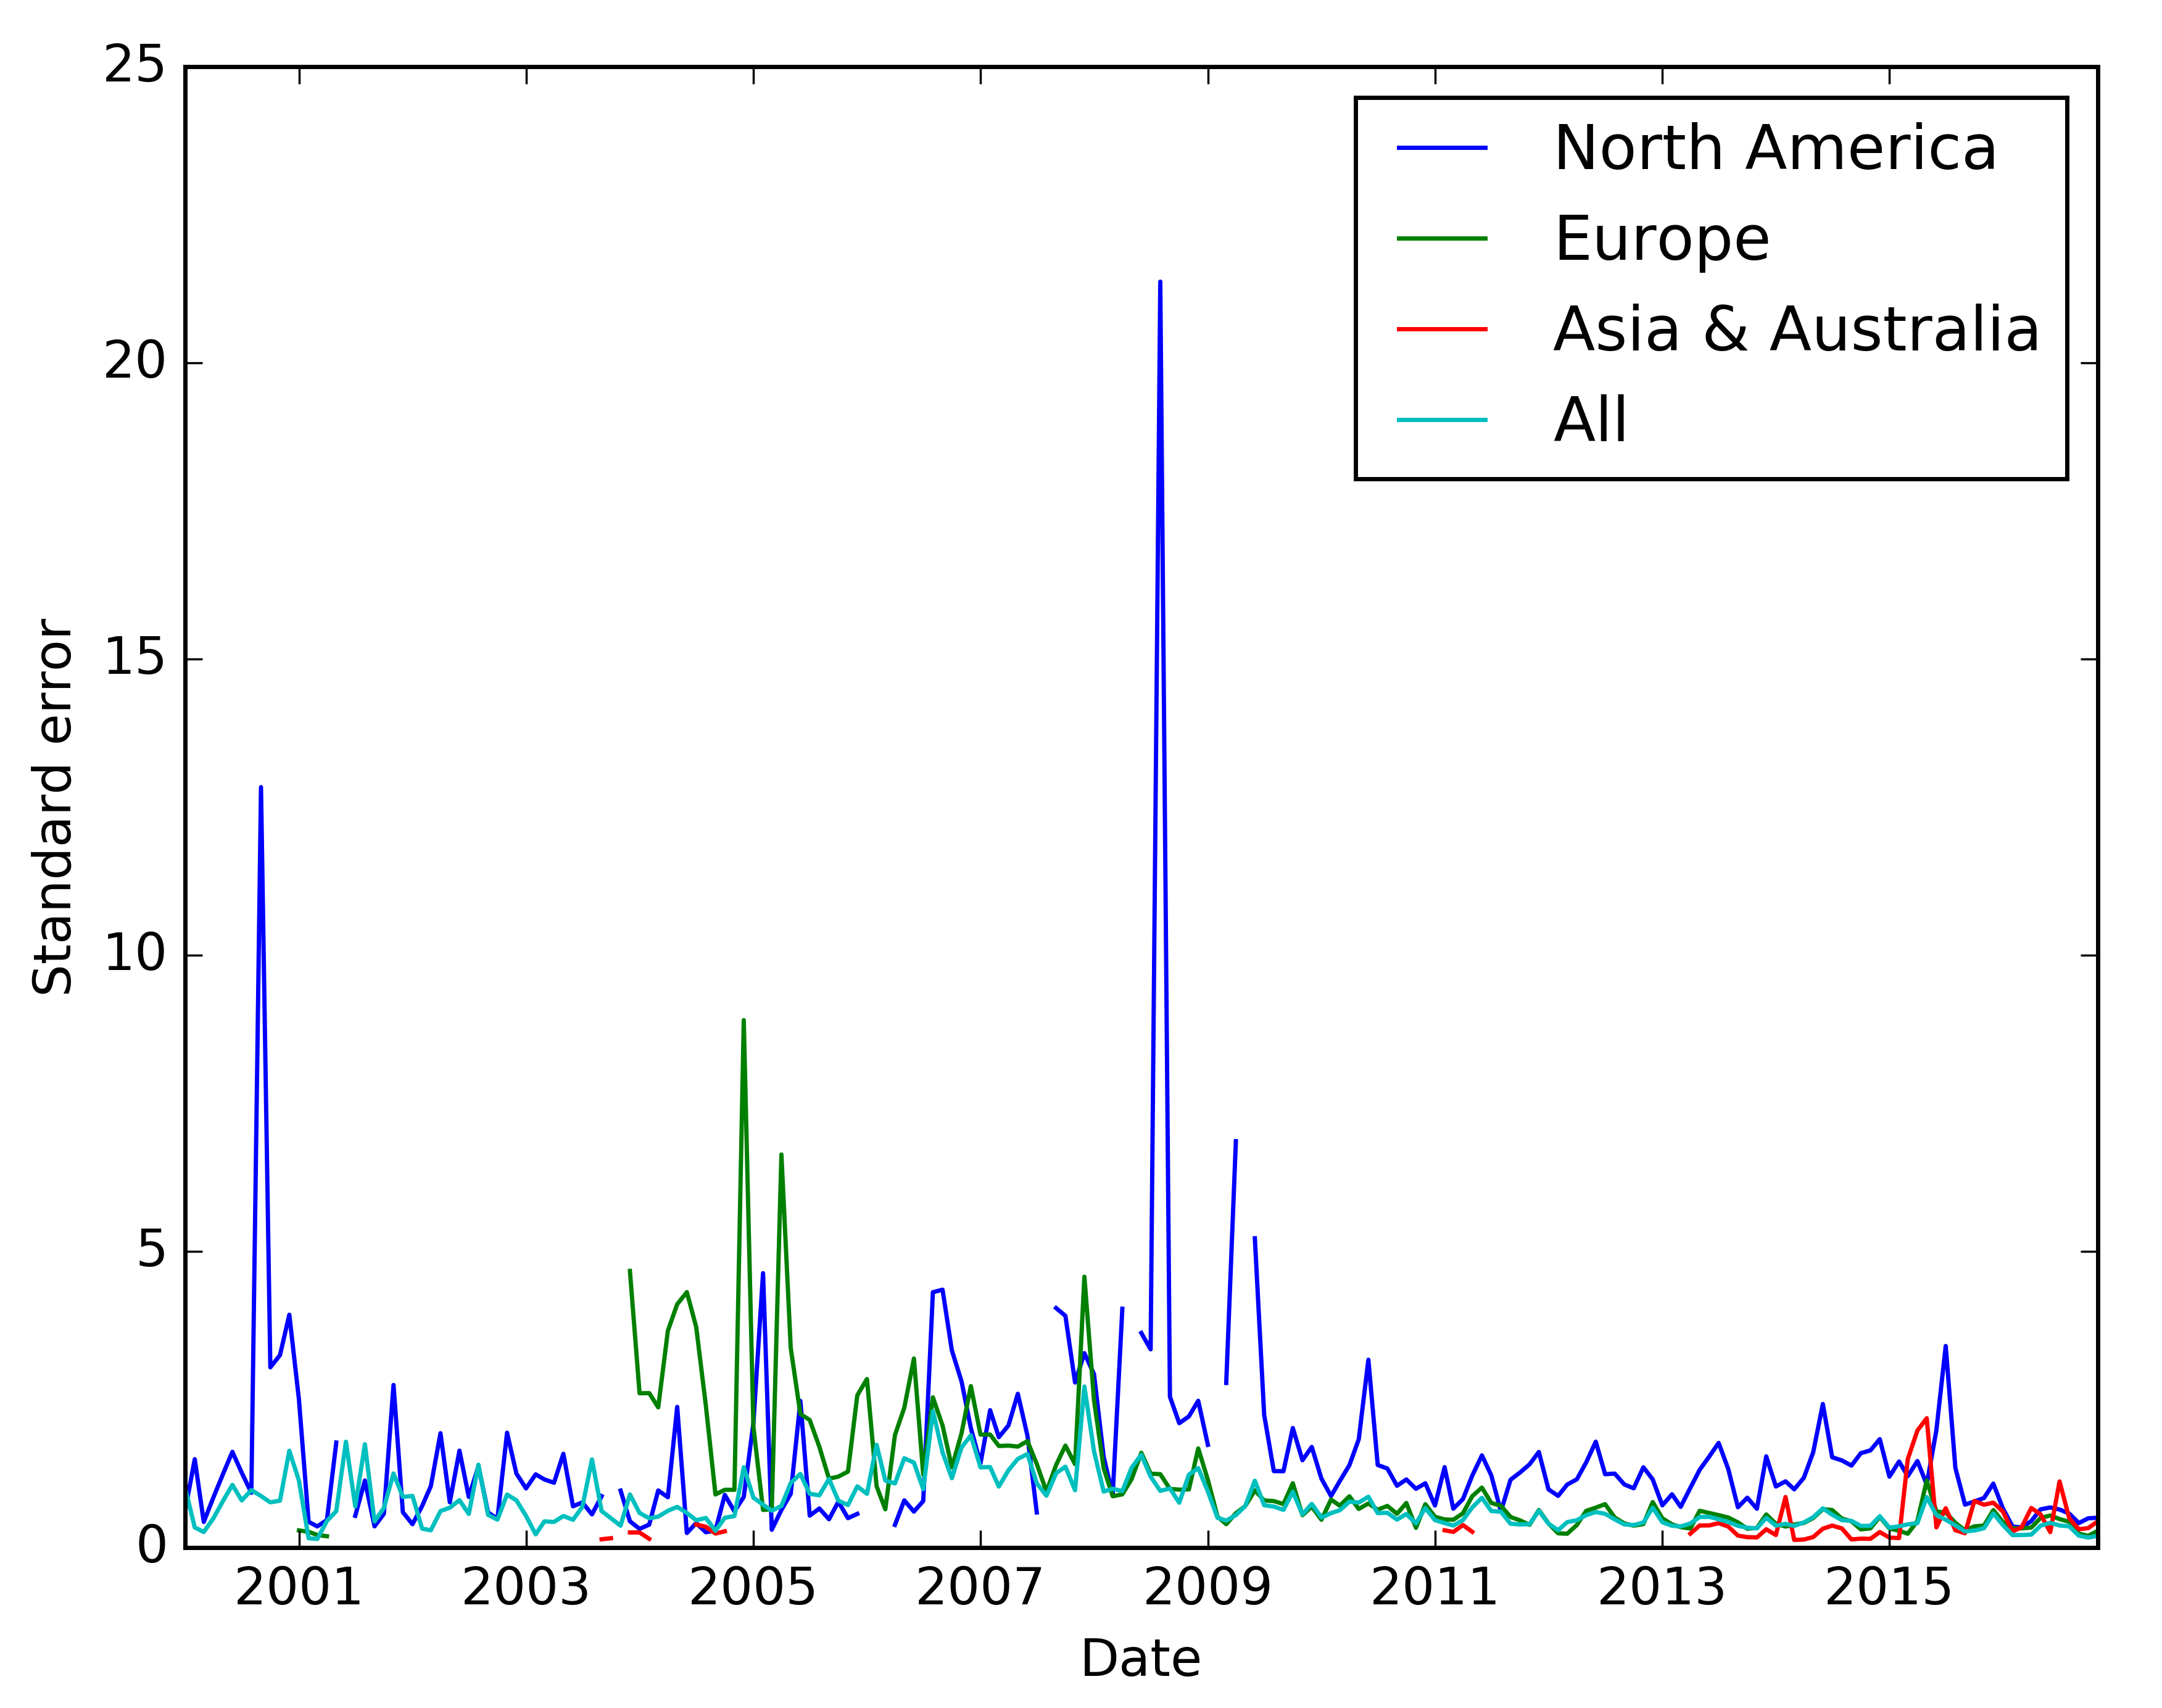
\includegraphics[width=\linewidth]{temporal/analyses/COMBINEDerr}
	\caption{Variation of standard error
		\label{fig:temp:err}}
\end{figure}
\paragraph{Skewness\\}
There does not appear to be a long term trend. The skewness is generally larger than 0, however it varies by $\sim$1, around 2000. This variation decreases over time, and the skewness appears to be closer to 0 for years 2005 onwards. There are anomalous results, but they are short term. For observers located in Europe, the skewness dips below 0 around 2005-2011 before fluctuating around 0 from 2011 onwards. This is the same for all categories; the values fluctuate around 0 between 2011 and 2015.
\begin{figure}[h!]
	\centering
	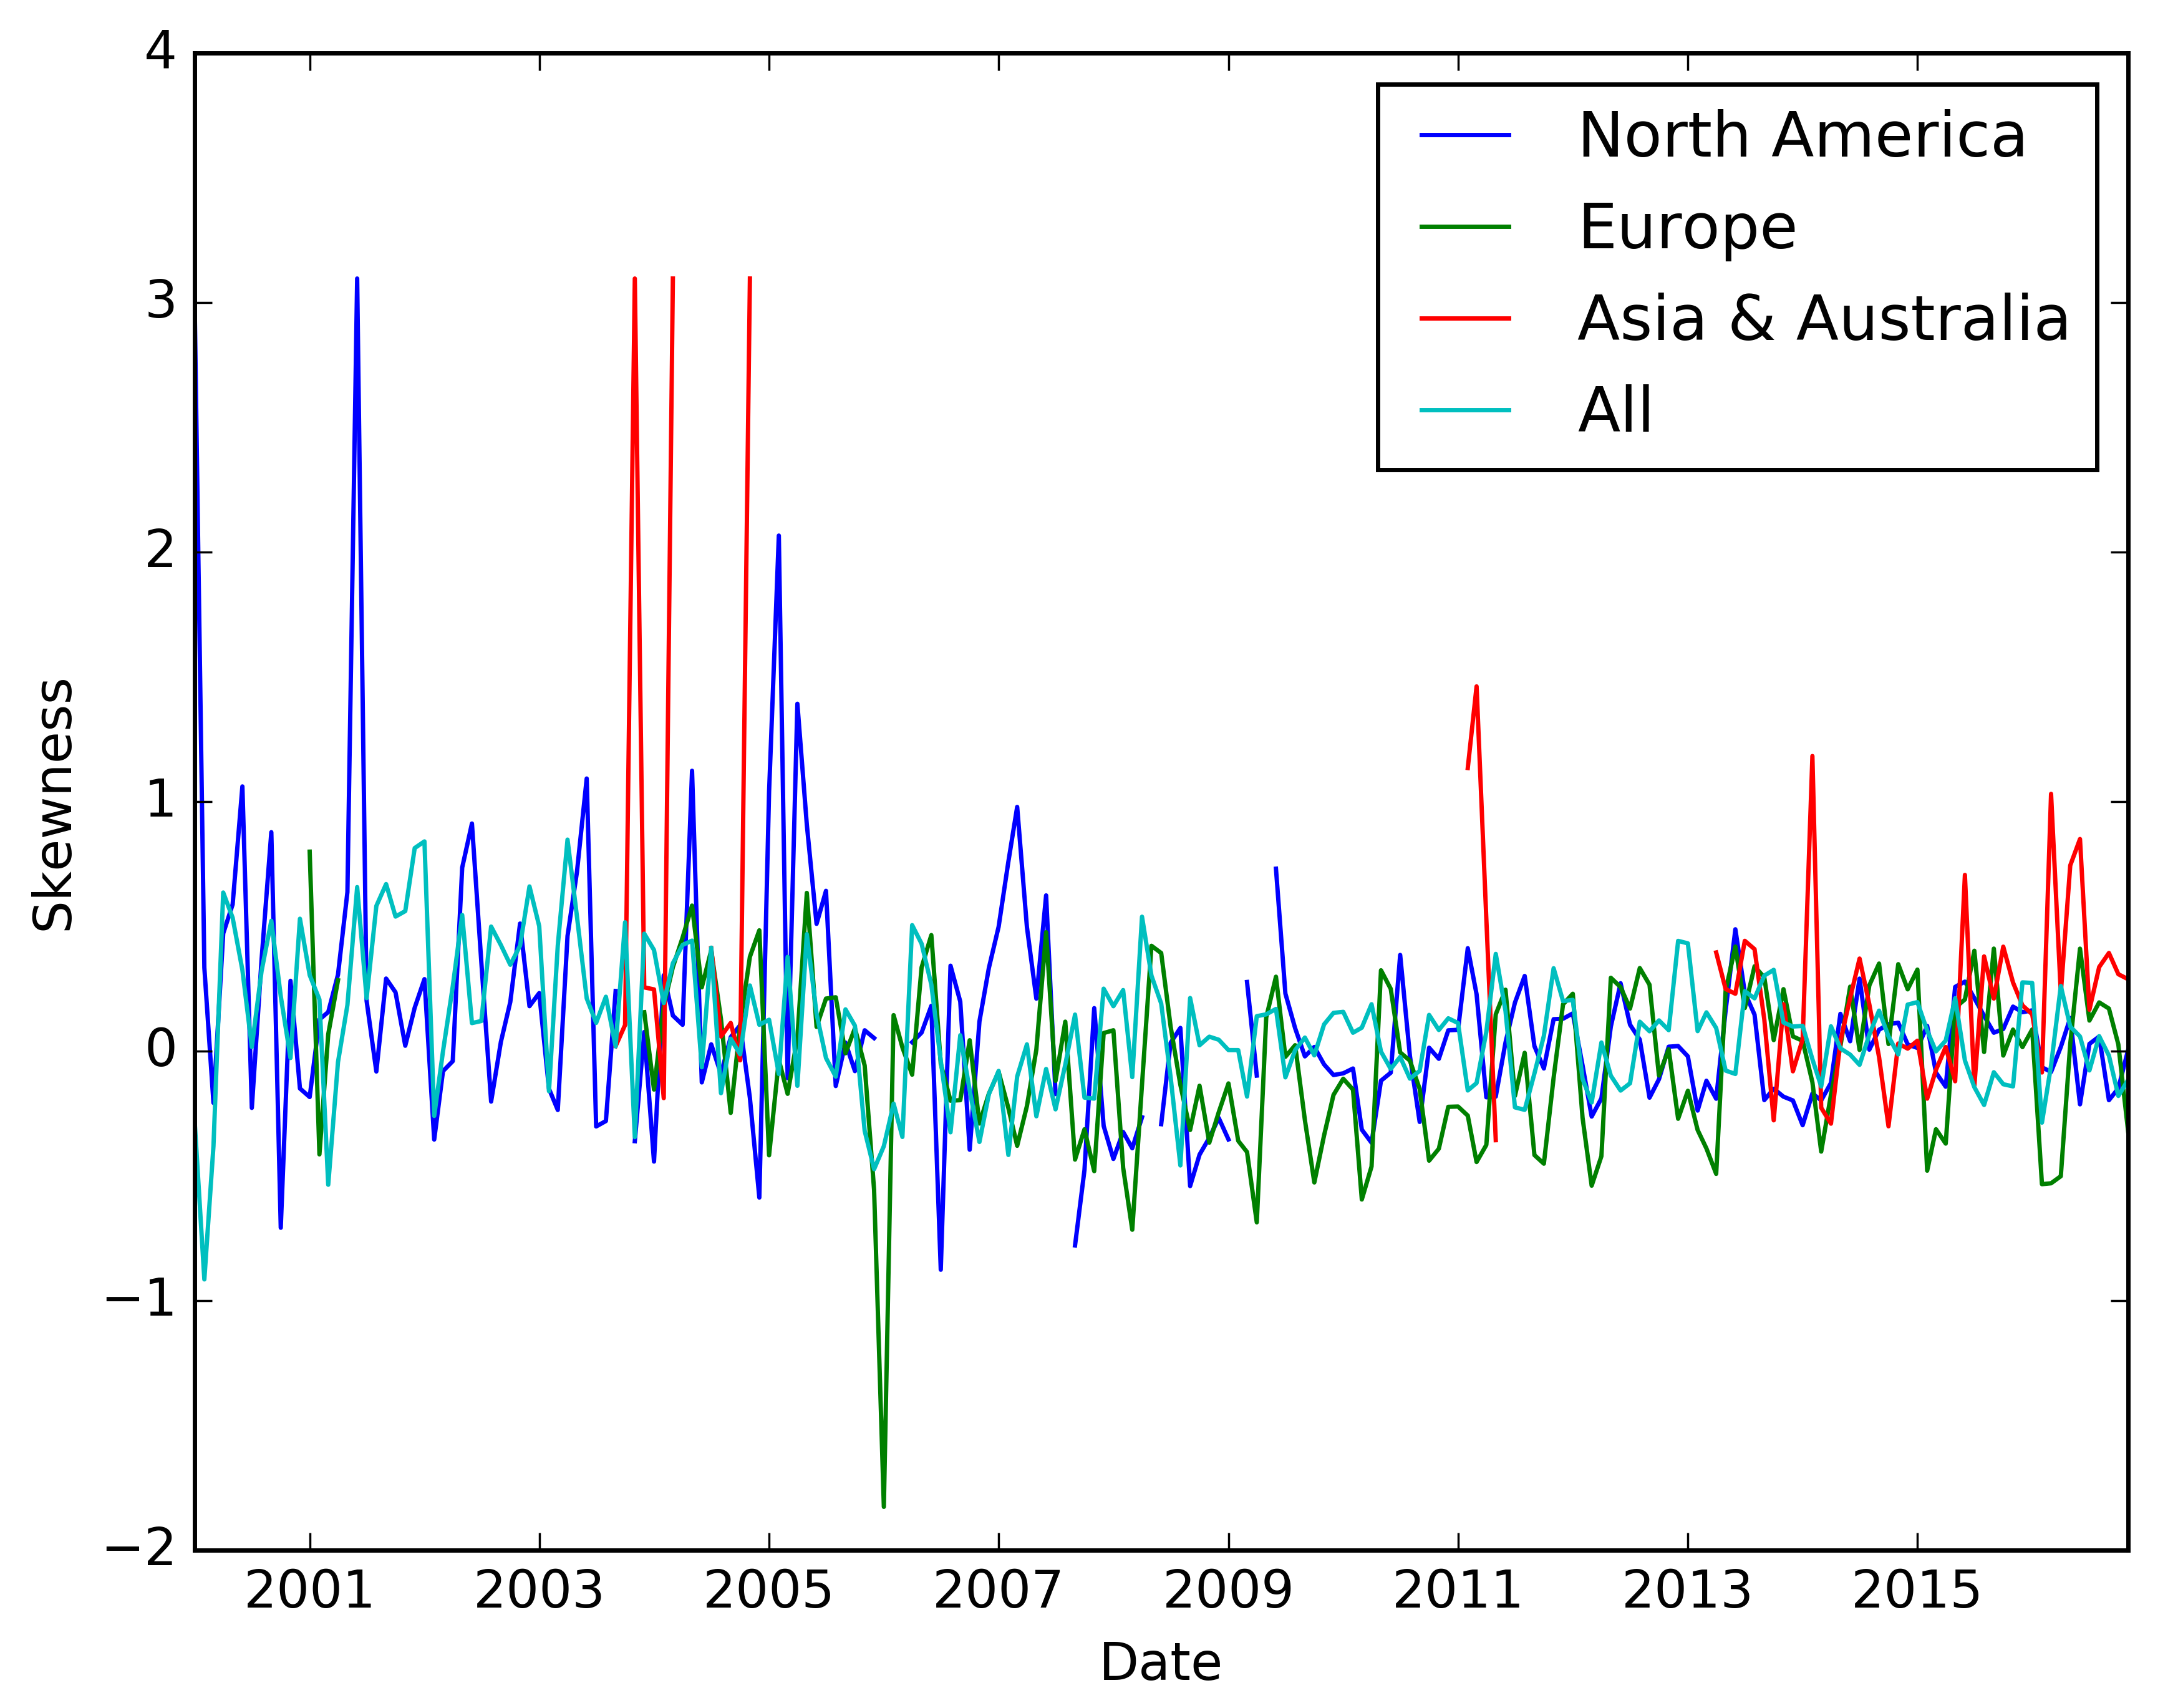
\includegraphics[width=\linewidth]{temporal/analyses/COMBINEDskew}
	\caption{Variation of skewness
		\label{fig:temp:skew}}
\end{figure}
\paragraph{Diurnal shift\\}
Between 2003 and 2007 there is a large amount of variation for observers in both Asia \& Australia, and North America. Towards more recent years, the variation is much smaller for all categories. The overall trend is not clear due to the large variation. Mostly, each category appears to fluctuate around certain values. For observers in Europe, this is $\sim$ 6, in Asia \& Australia the values fluctuate around $\sim$ 18, and in North America, around $\sim$12.
\begin{figure}[h!]
	\centering
	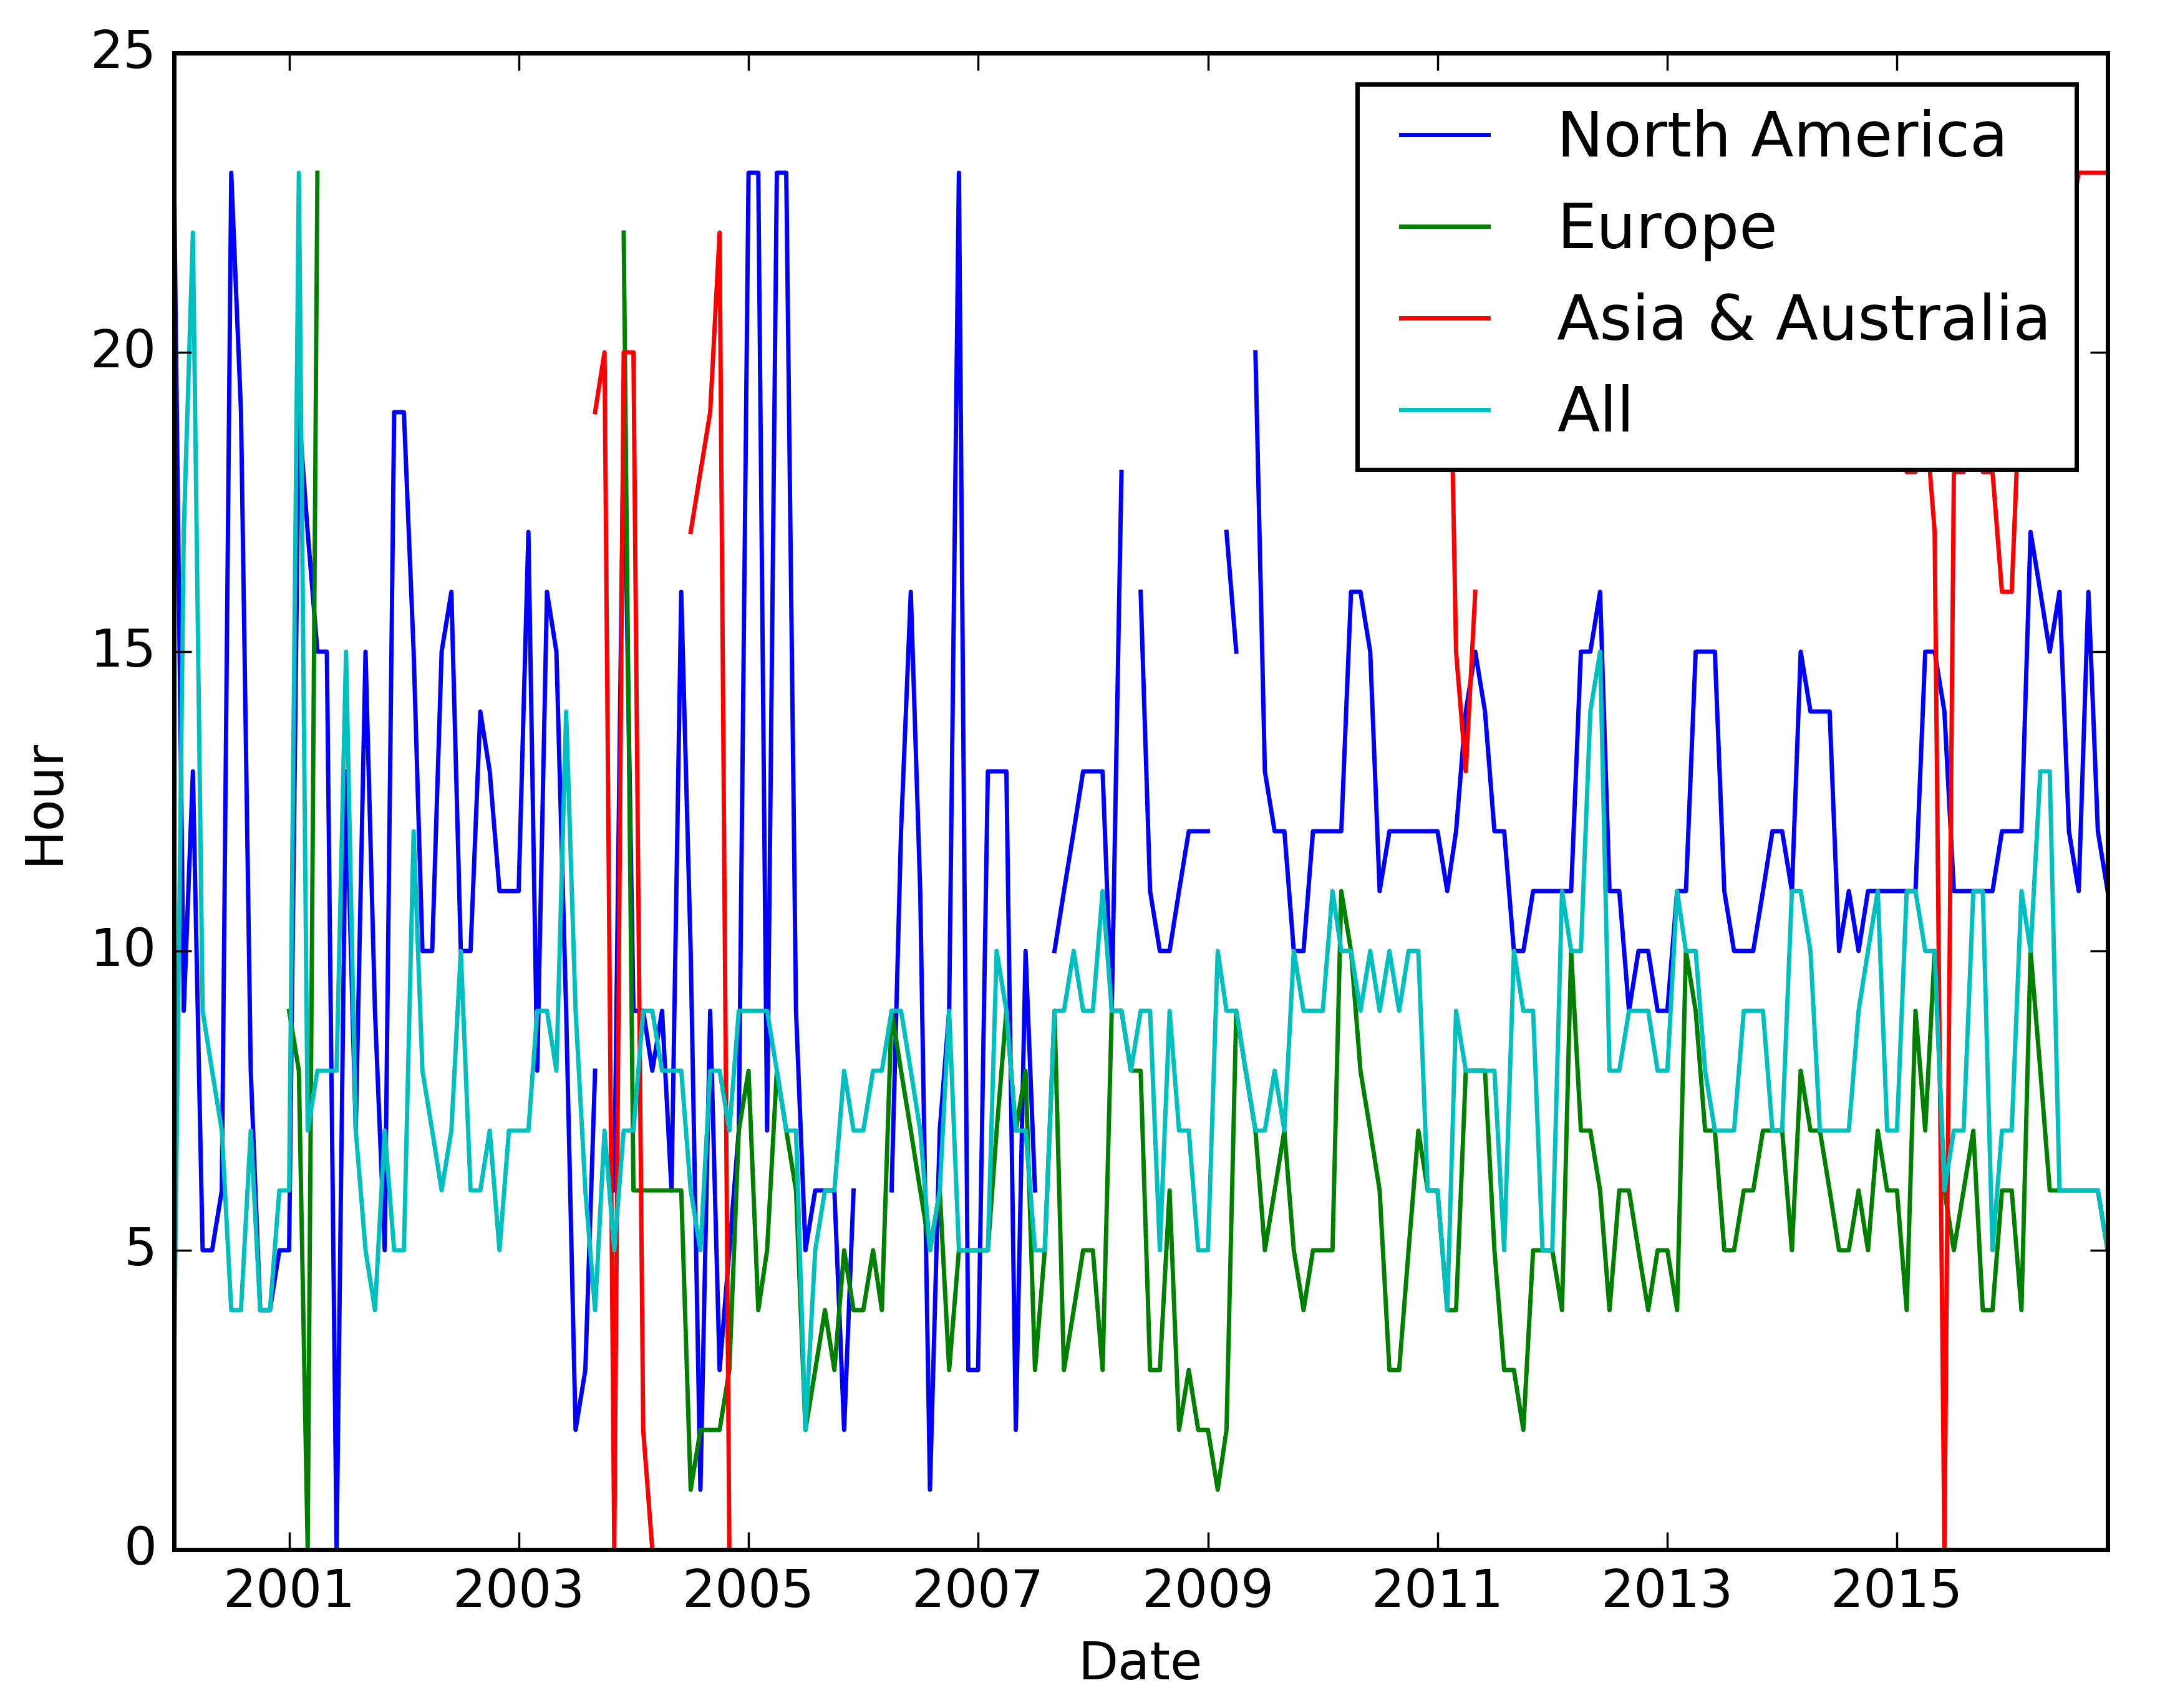
\includegraphics[width=\linewidth]{temporal/analyses/COMBINEDpeak}
	\caption{Variation of peak hour of diurnal shift
		\label{fig:temp:peak}}
\end{figure}
During the periods with the most fluctuation in figure~\ref{fig:temp:peak}, the sum of the parameter covariance, indicating how well a sine function fits the data, is greatest. The mean fit, across all observers, is relatively low throughout the years available, however there is again a noticeable increase between 2005 and 2010, which fits in with increases \& decreases in other analyses. The fit is closer to 0 in recent years, for all categories other than North America, though this category does decrease too.
\begin{figure}[h!]
	\centering
	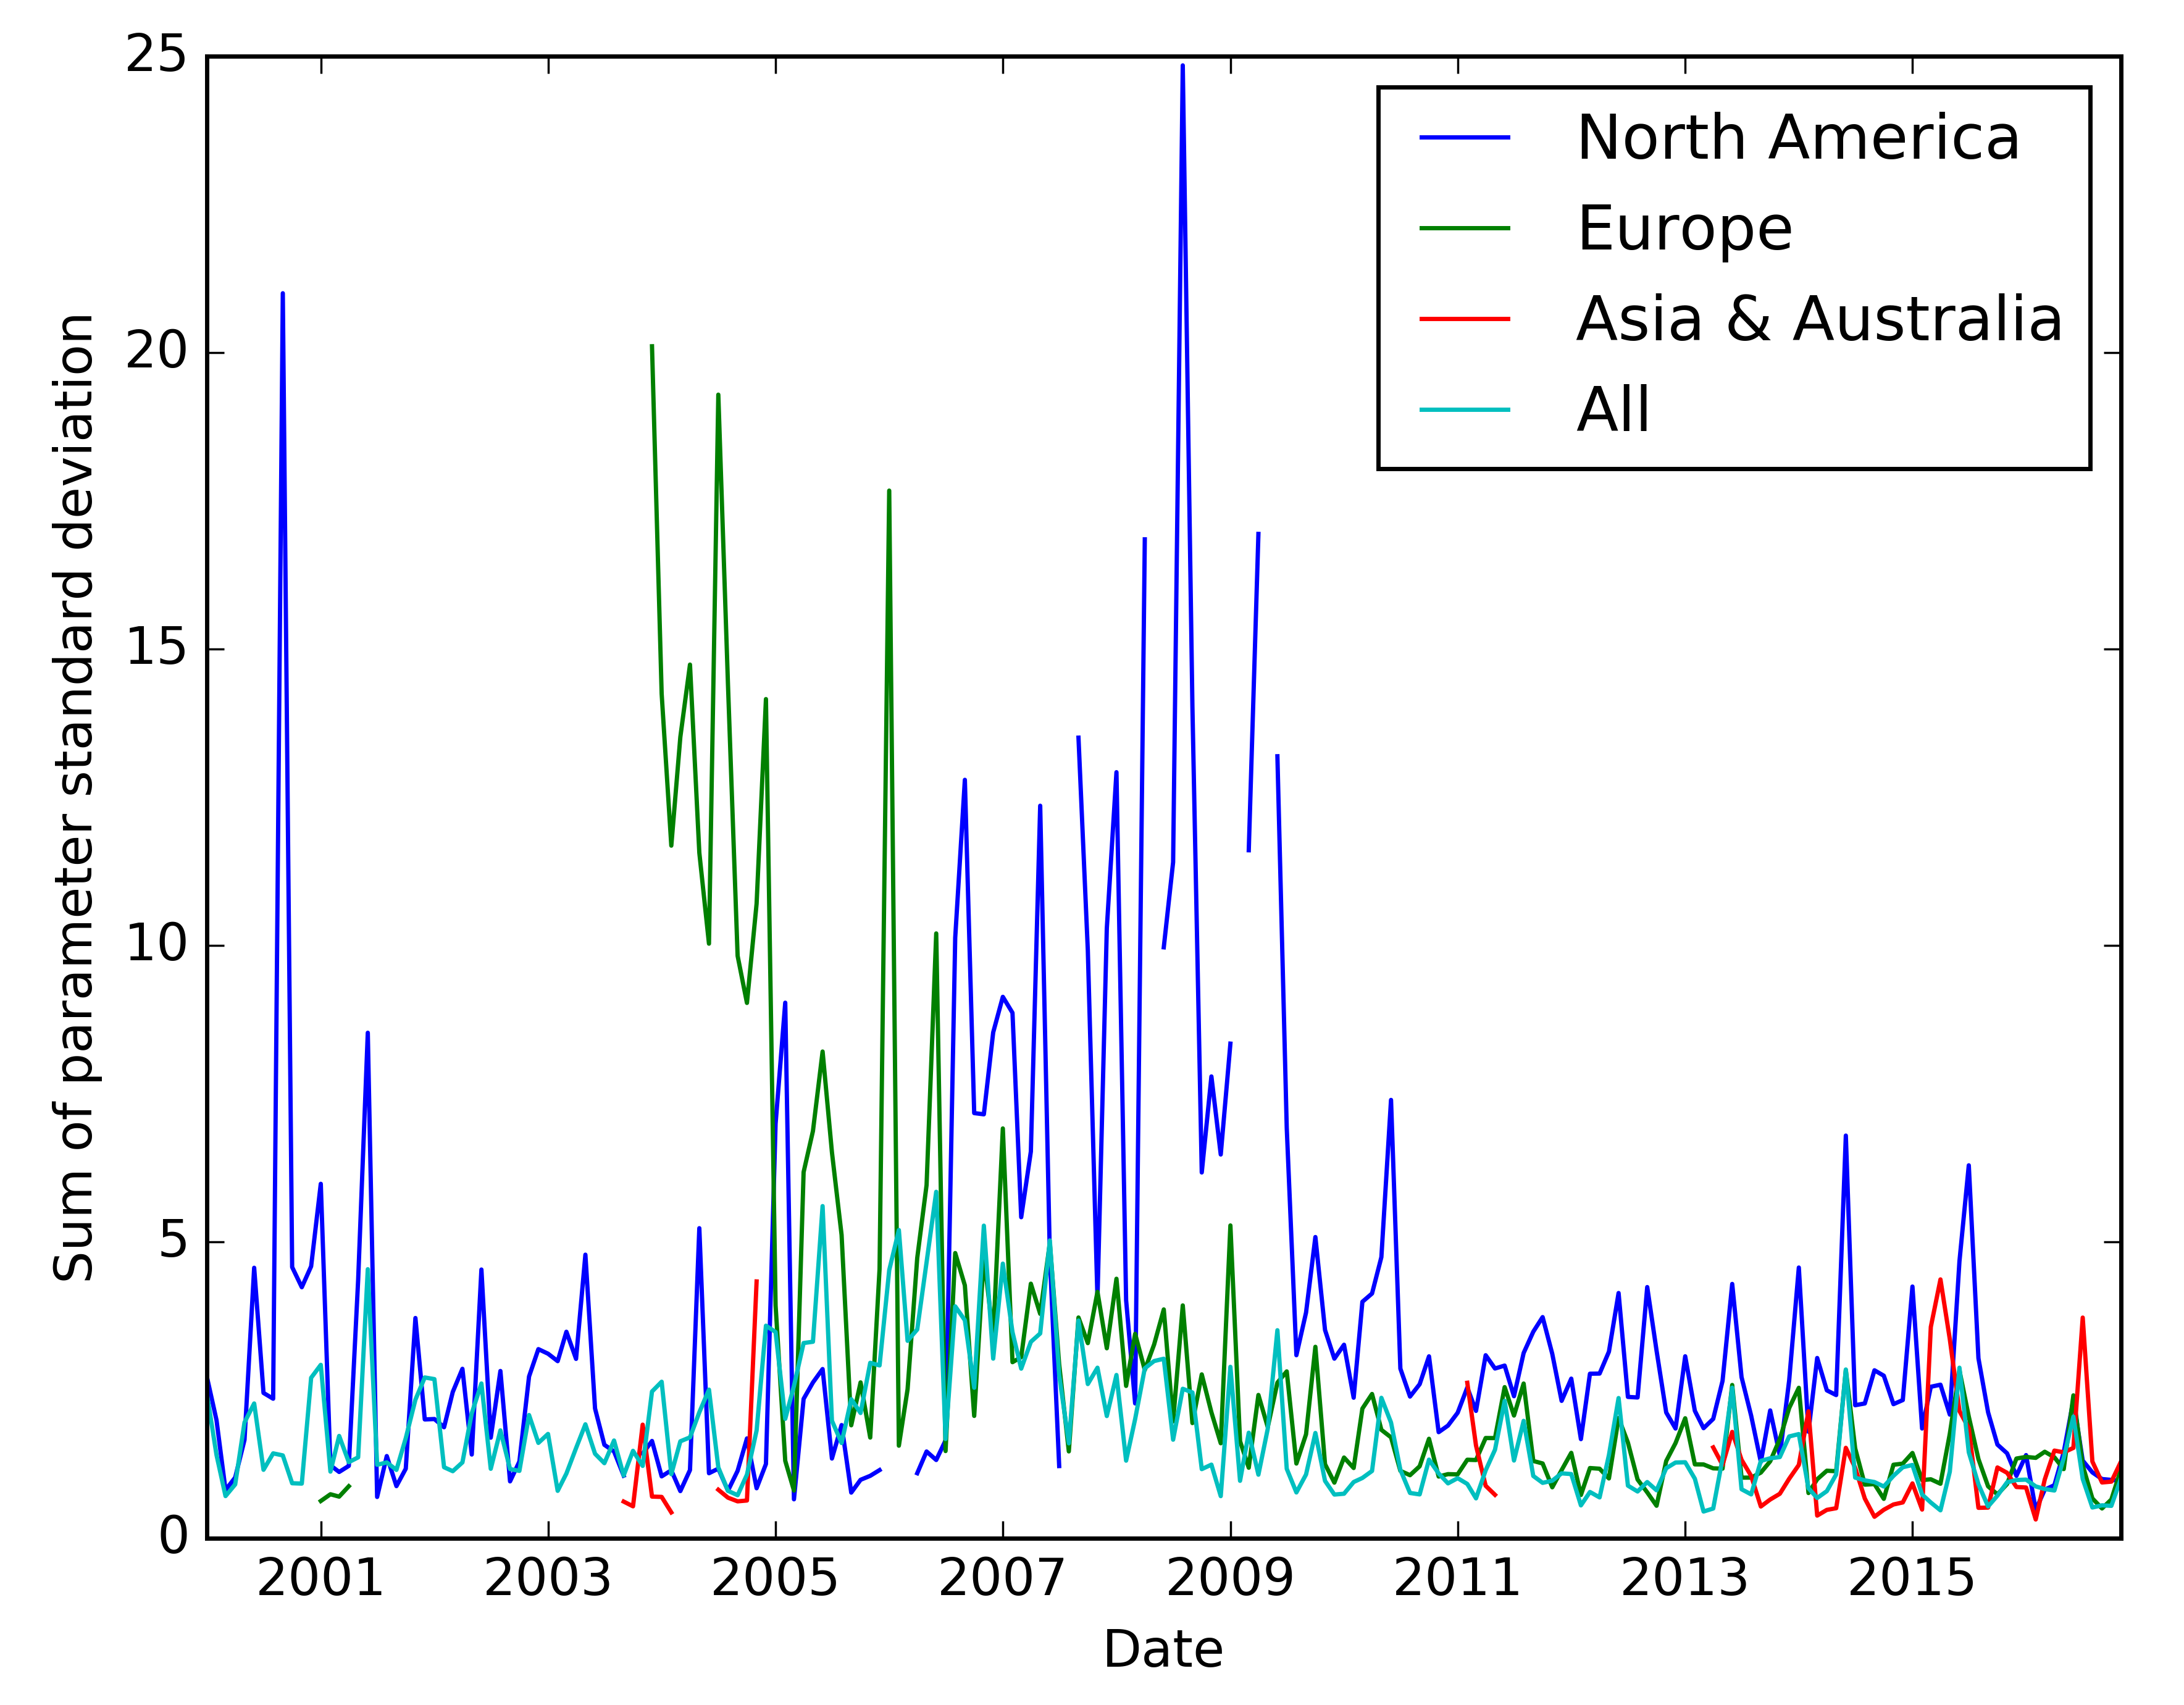
\includegraphics[width=\linewidth]{temporal/analyses/COMBINEDfit}
	\caption{Variation of fit to optimal sine function for diurnal shift
		\label{fig:temp:fit}}
\end{figure}

\subsection{Monthly scale variation}
The variation over the course of a month is shown in figure~\ref{fig:temp:day}. There is no overall trend throughout a month. There is no overall increase or decrease, though there is a slight increase around the 13th day in the month.
\begin{figure}[h!]
	\centering
	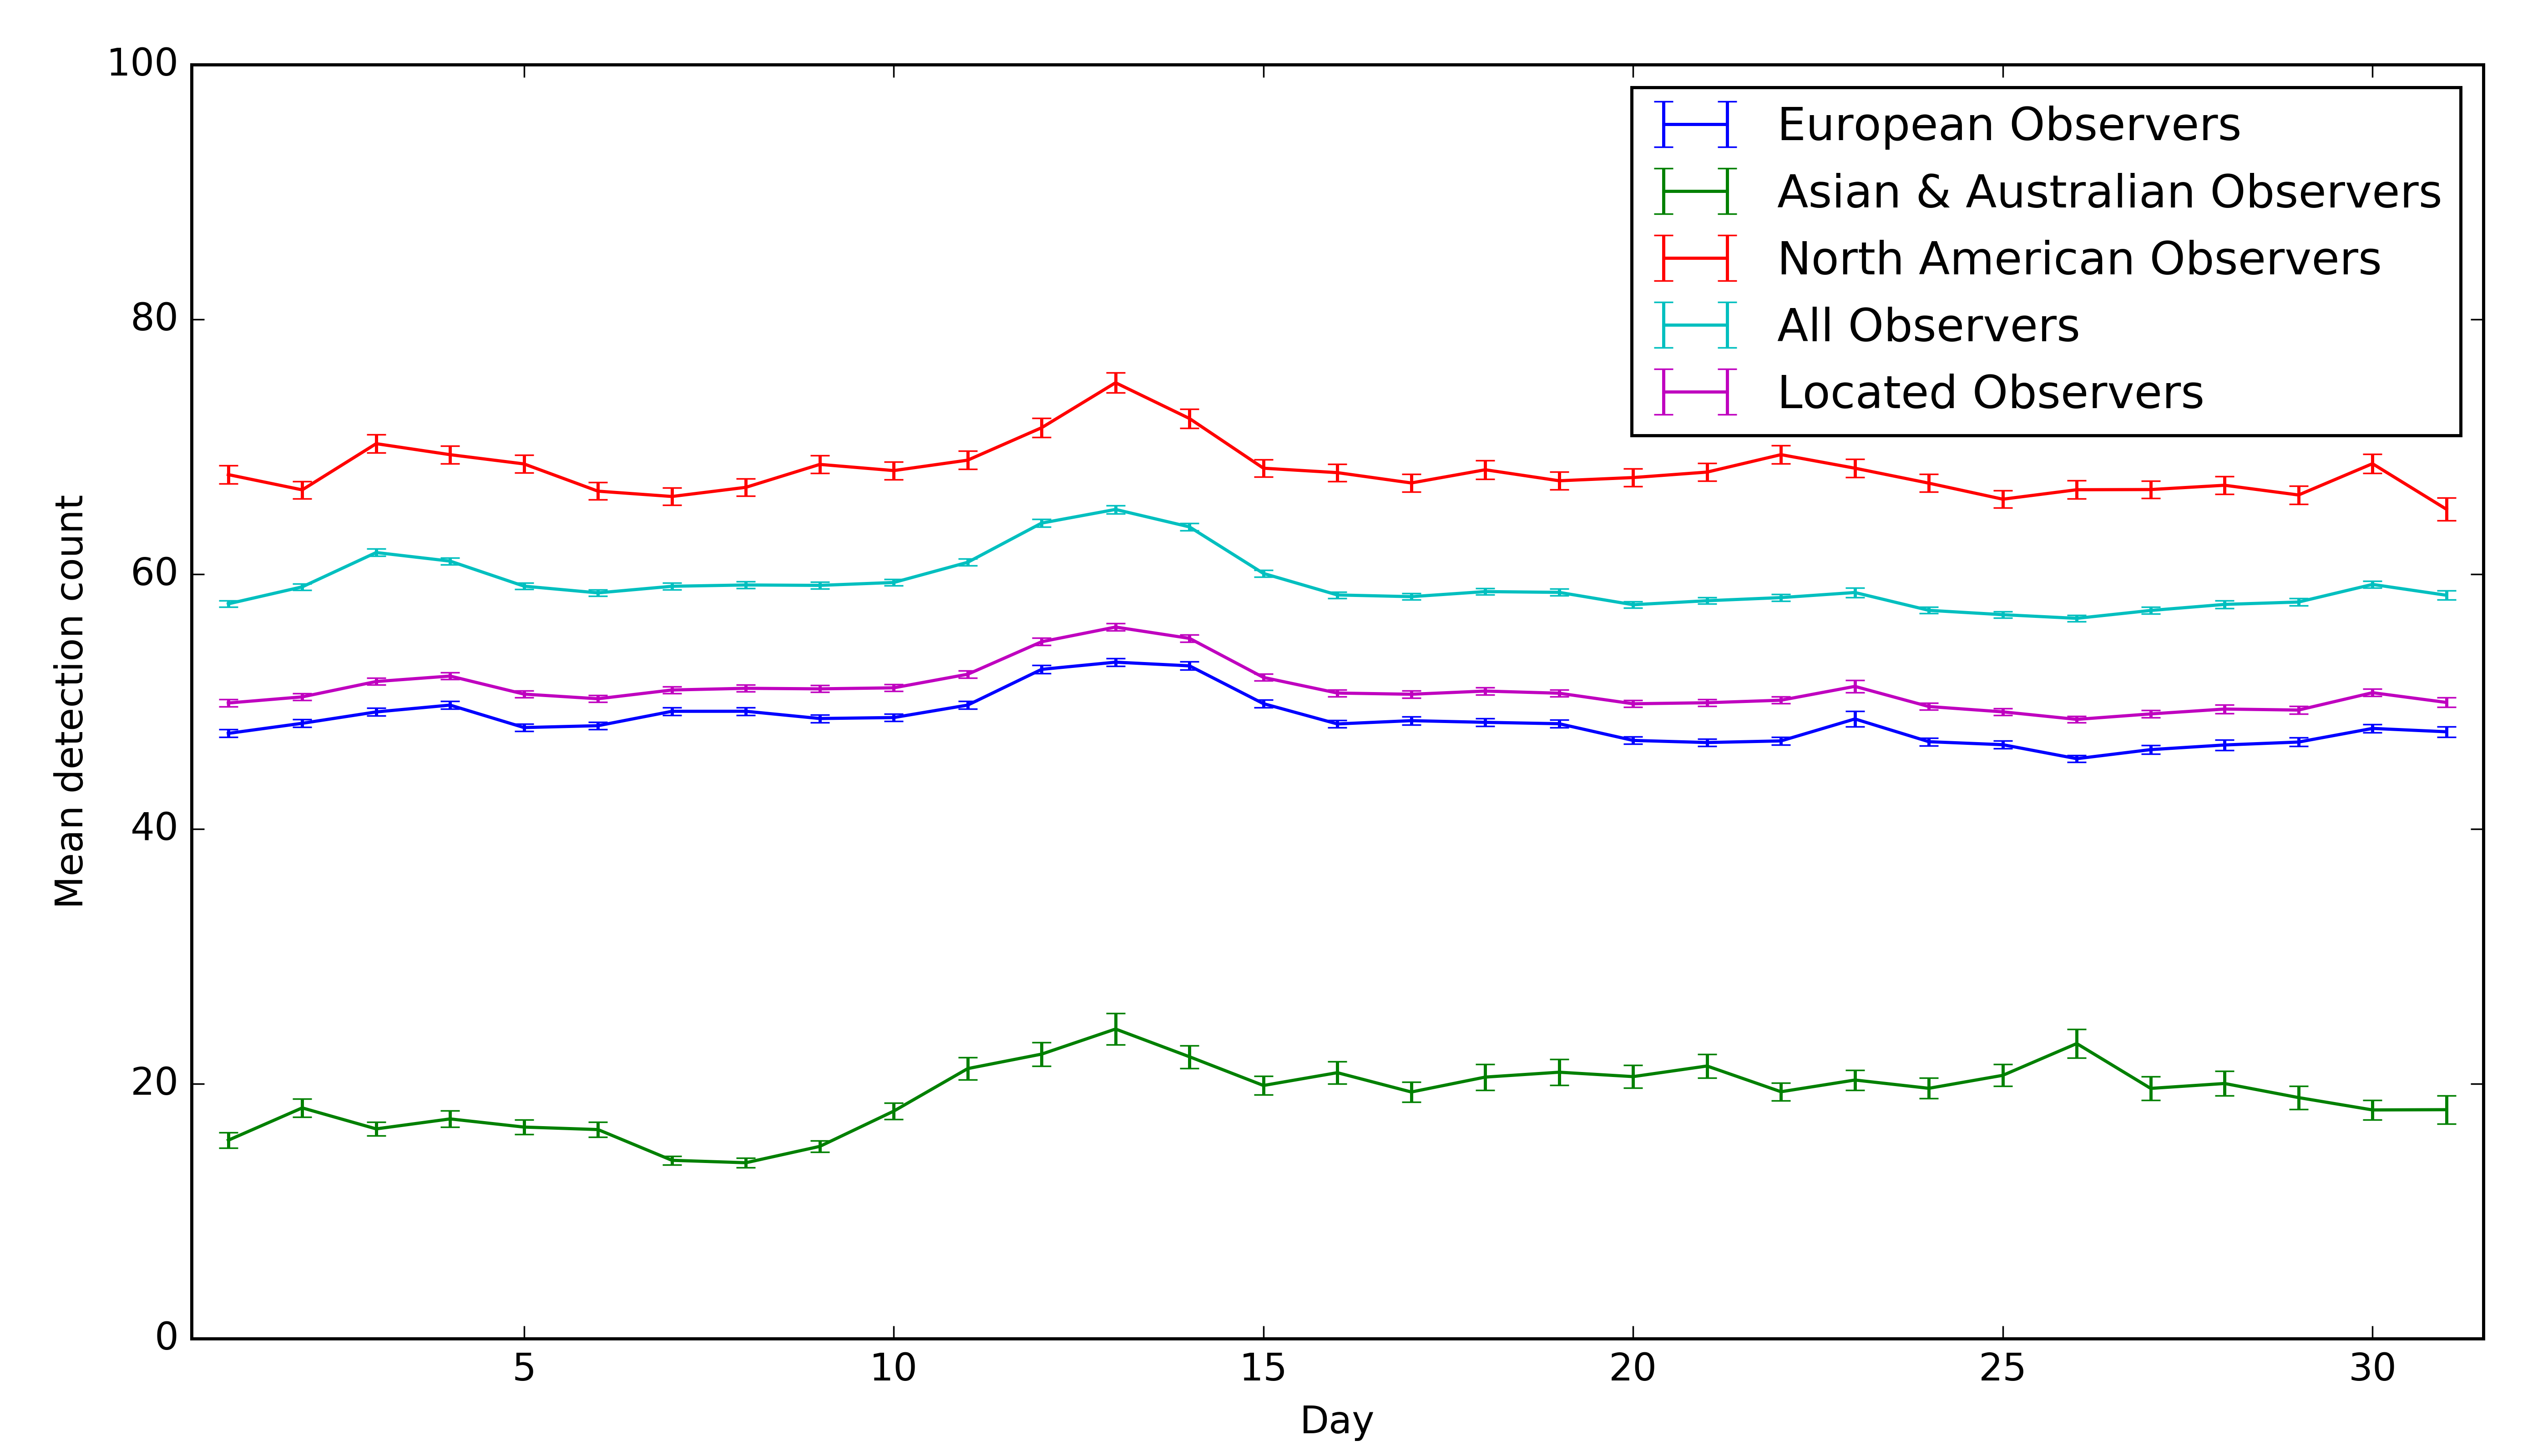
\includegraphics[width=\linewidth]{temporal/Dcombined}
	\caption{Variation in mean hourly detection count over a month
		\label{fig:temp:day}}
\end{figure}
\subsection{Annual scale variation}
There is a clear increase from the beginning of a year to the end, for all categories other than Asia \& Australia. From January to February, there is a small decrease, followed by an increase until June. This is followed by a small decrease of $\sim$ 10 detections an hour, until August. The mean hourly detection count then remains roughly constant until the end of the year. This is the same for all categories other than Asia \& Australia. For this category, there is an increase in April and May, and then a decrease and a constant hourly count for the rest of the year.
\begin{figure}[h!]
	\centering
	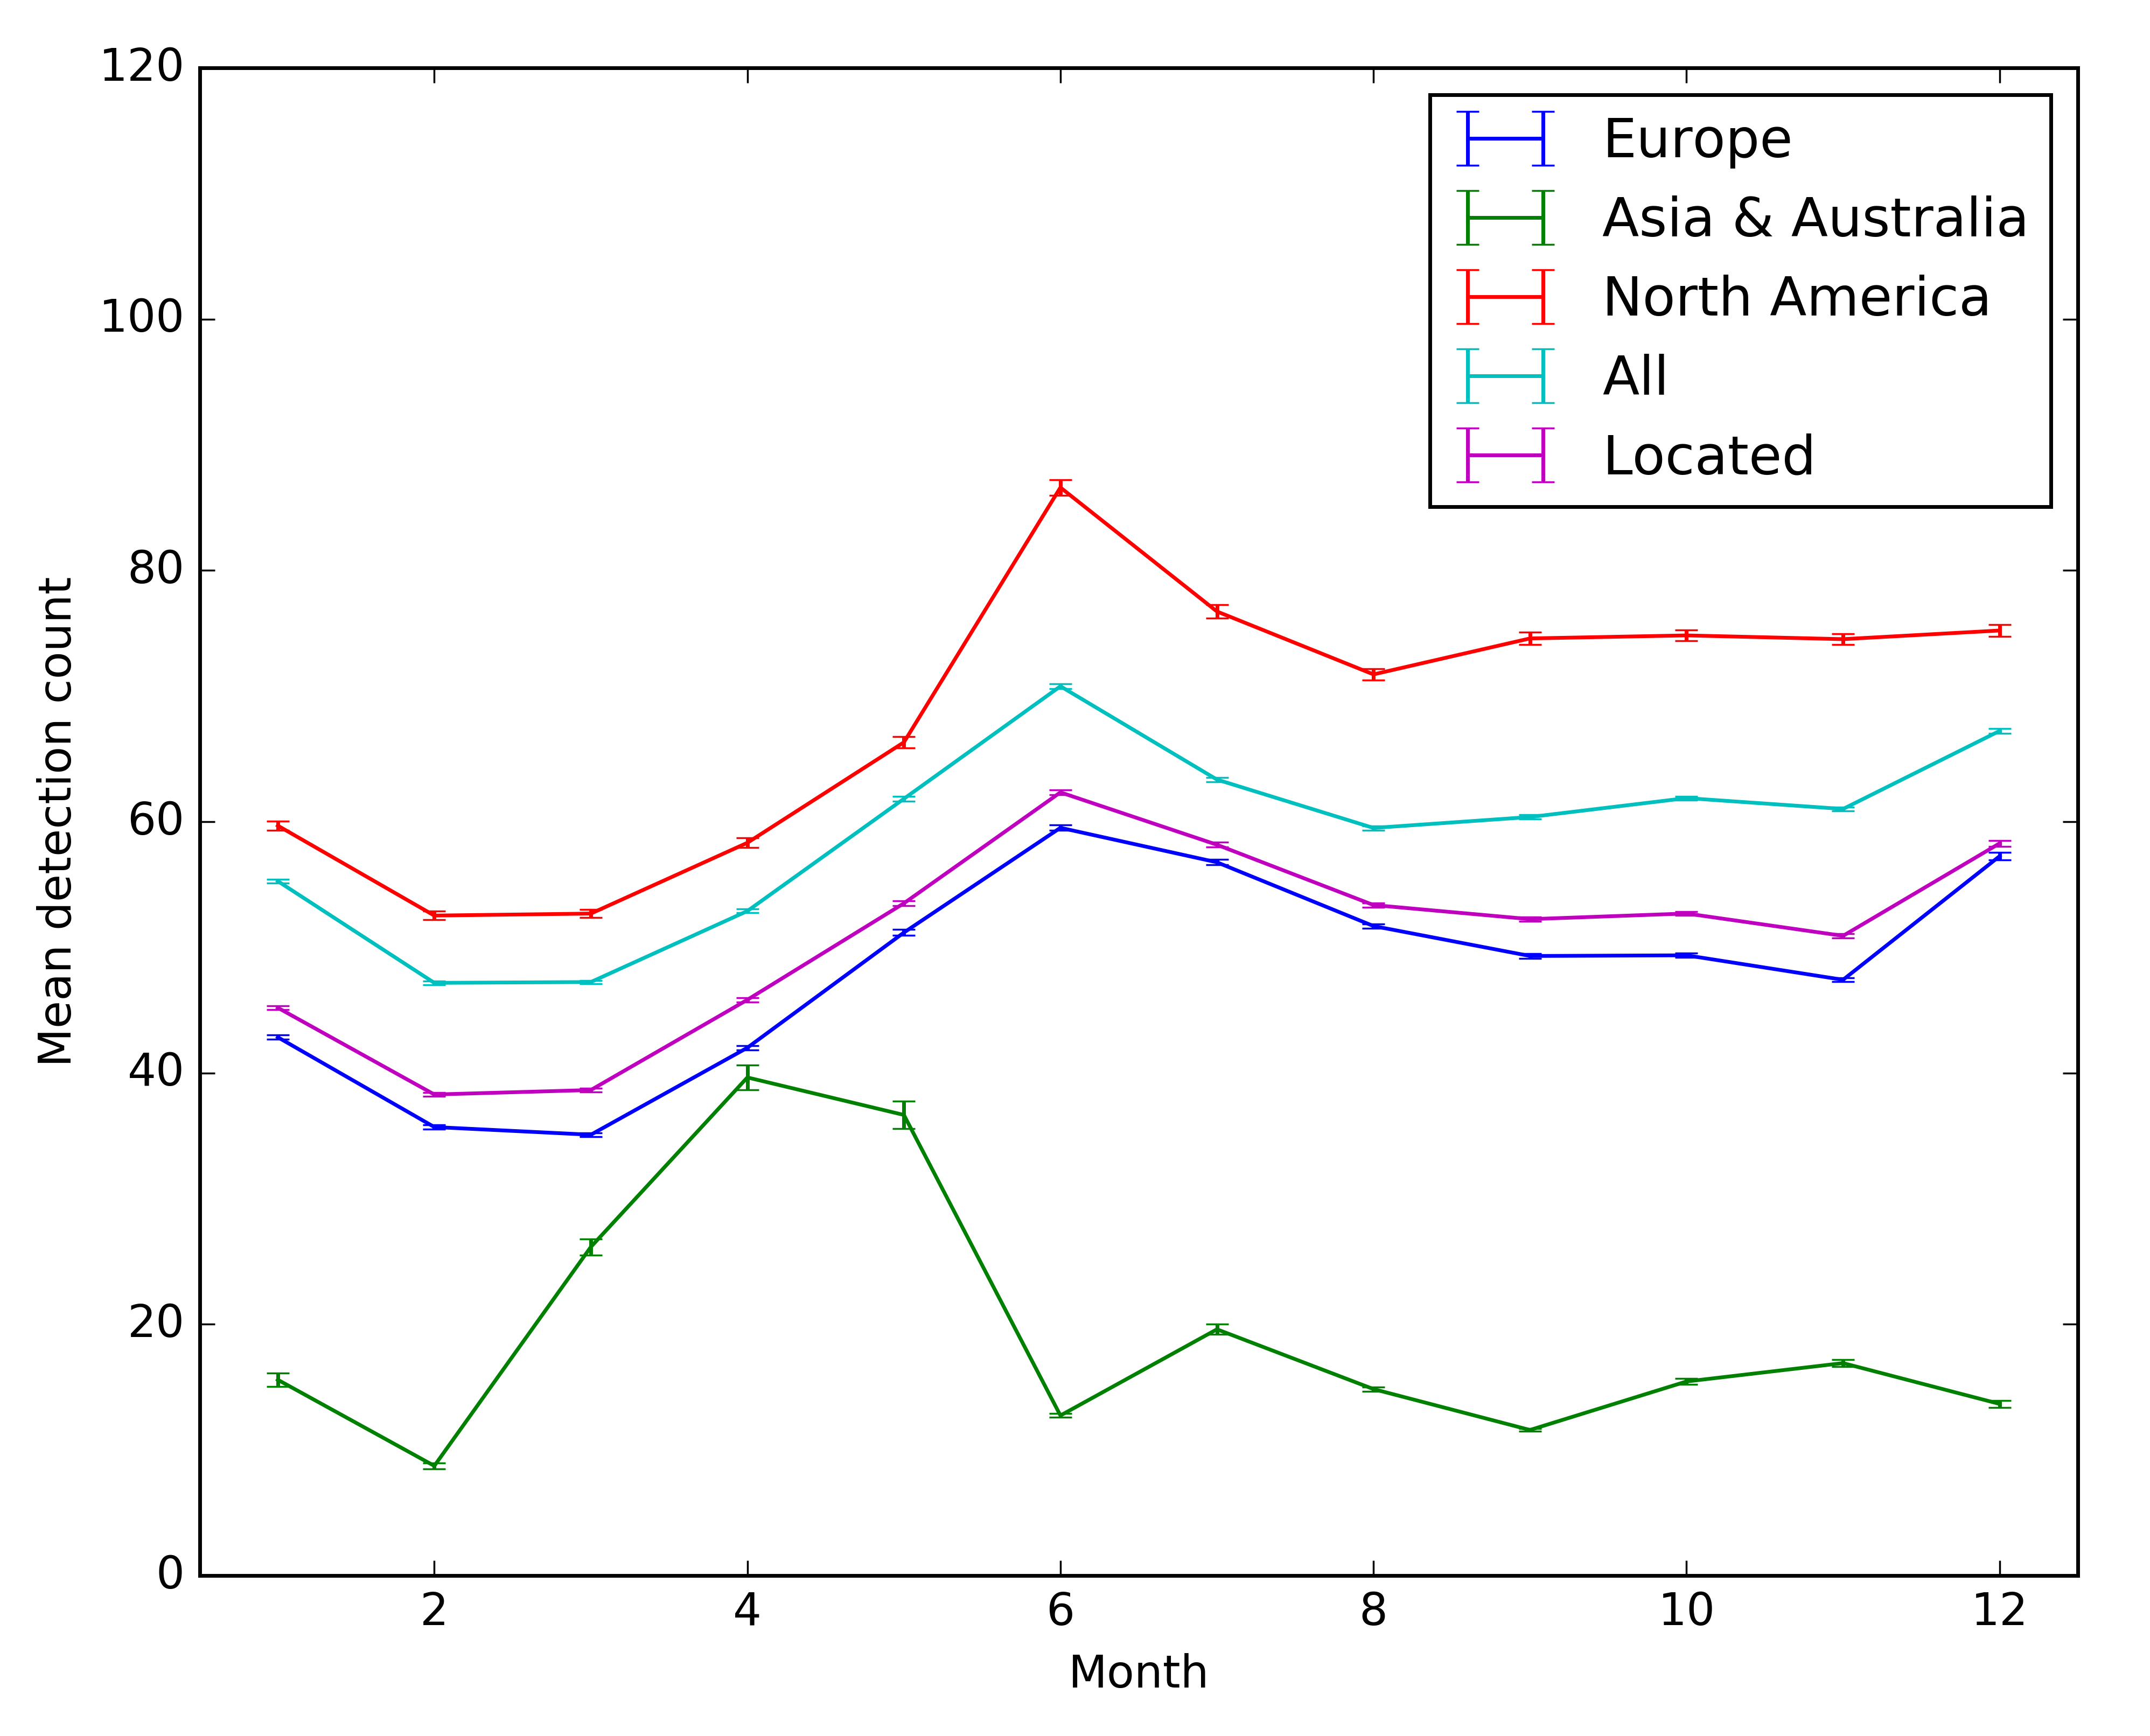
\includegraphics[width=\linewidth]{temporal/Mcombined}
	\caption{Variation in mean hourly detection count over a year
		\label{fig:temp:month}}
\end{figure}
\subsection{Variation since 2000}
Between 2003 and 2011 there is a dramatic increase in the mean hourly detection count across an entire year. This increase is on the order of $\sim$ 2 times, from $\sim$ 60 to $\sim$ 120. This increase is out of phase by 1 year for the North American category. Once the count returns to $\sim$ 60, it remains there from 2011 to 2016. There is no data available for the Asia \& Australia category for the maximum period so it is not known if the same increase is seen, however the category containing observers from the entire world exhibits the increase. Whilst the North American category has another peak in 2003, the standard error is much larger.
\begin{figure}[h!]
	\centering
	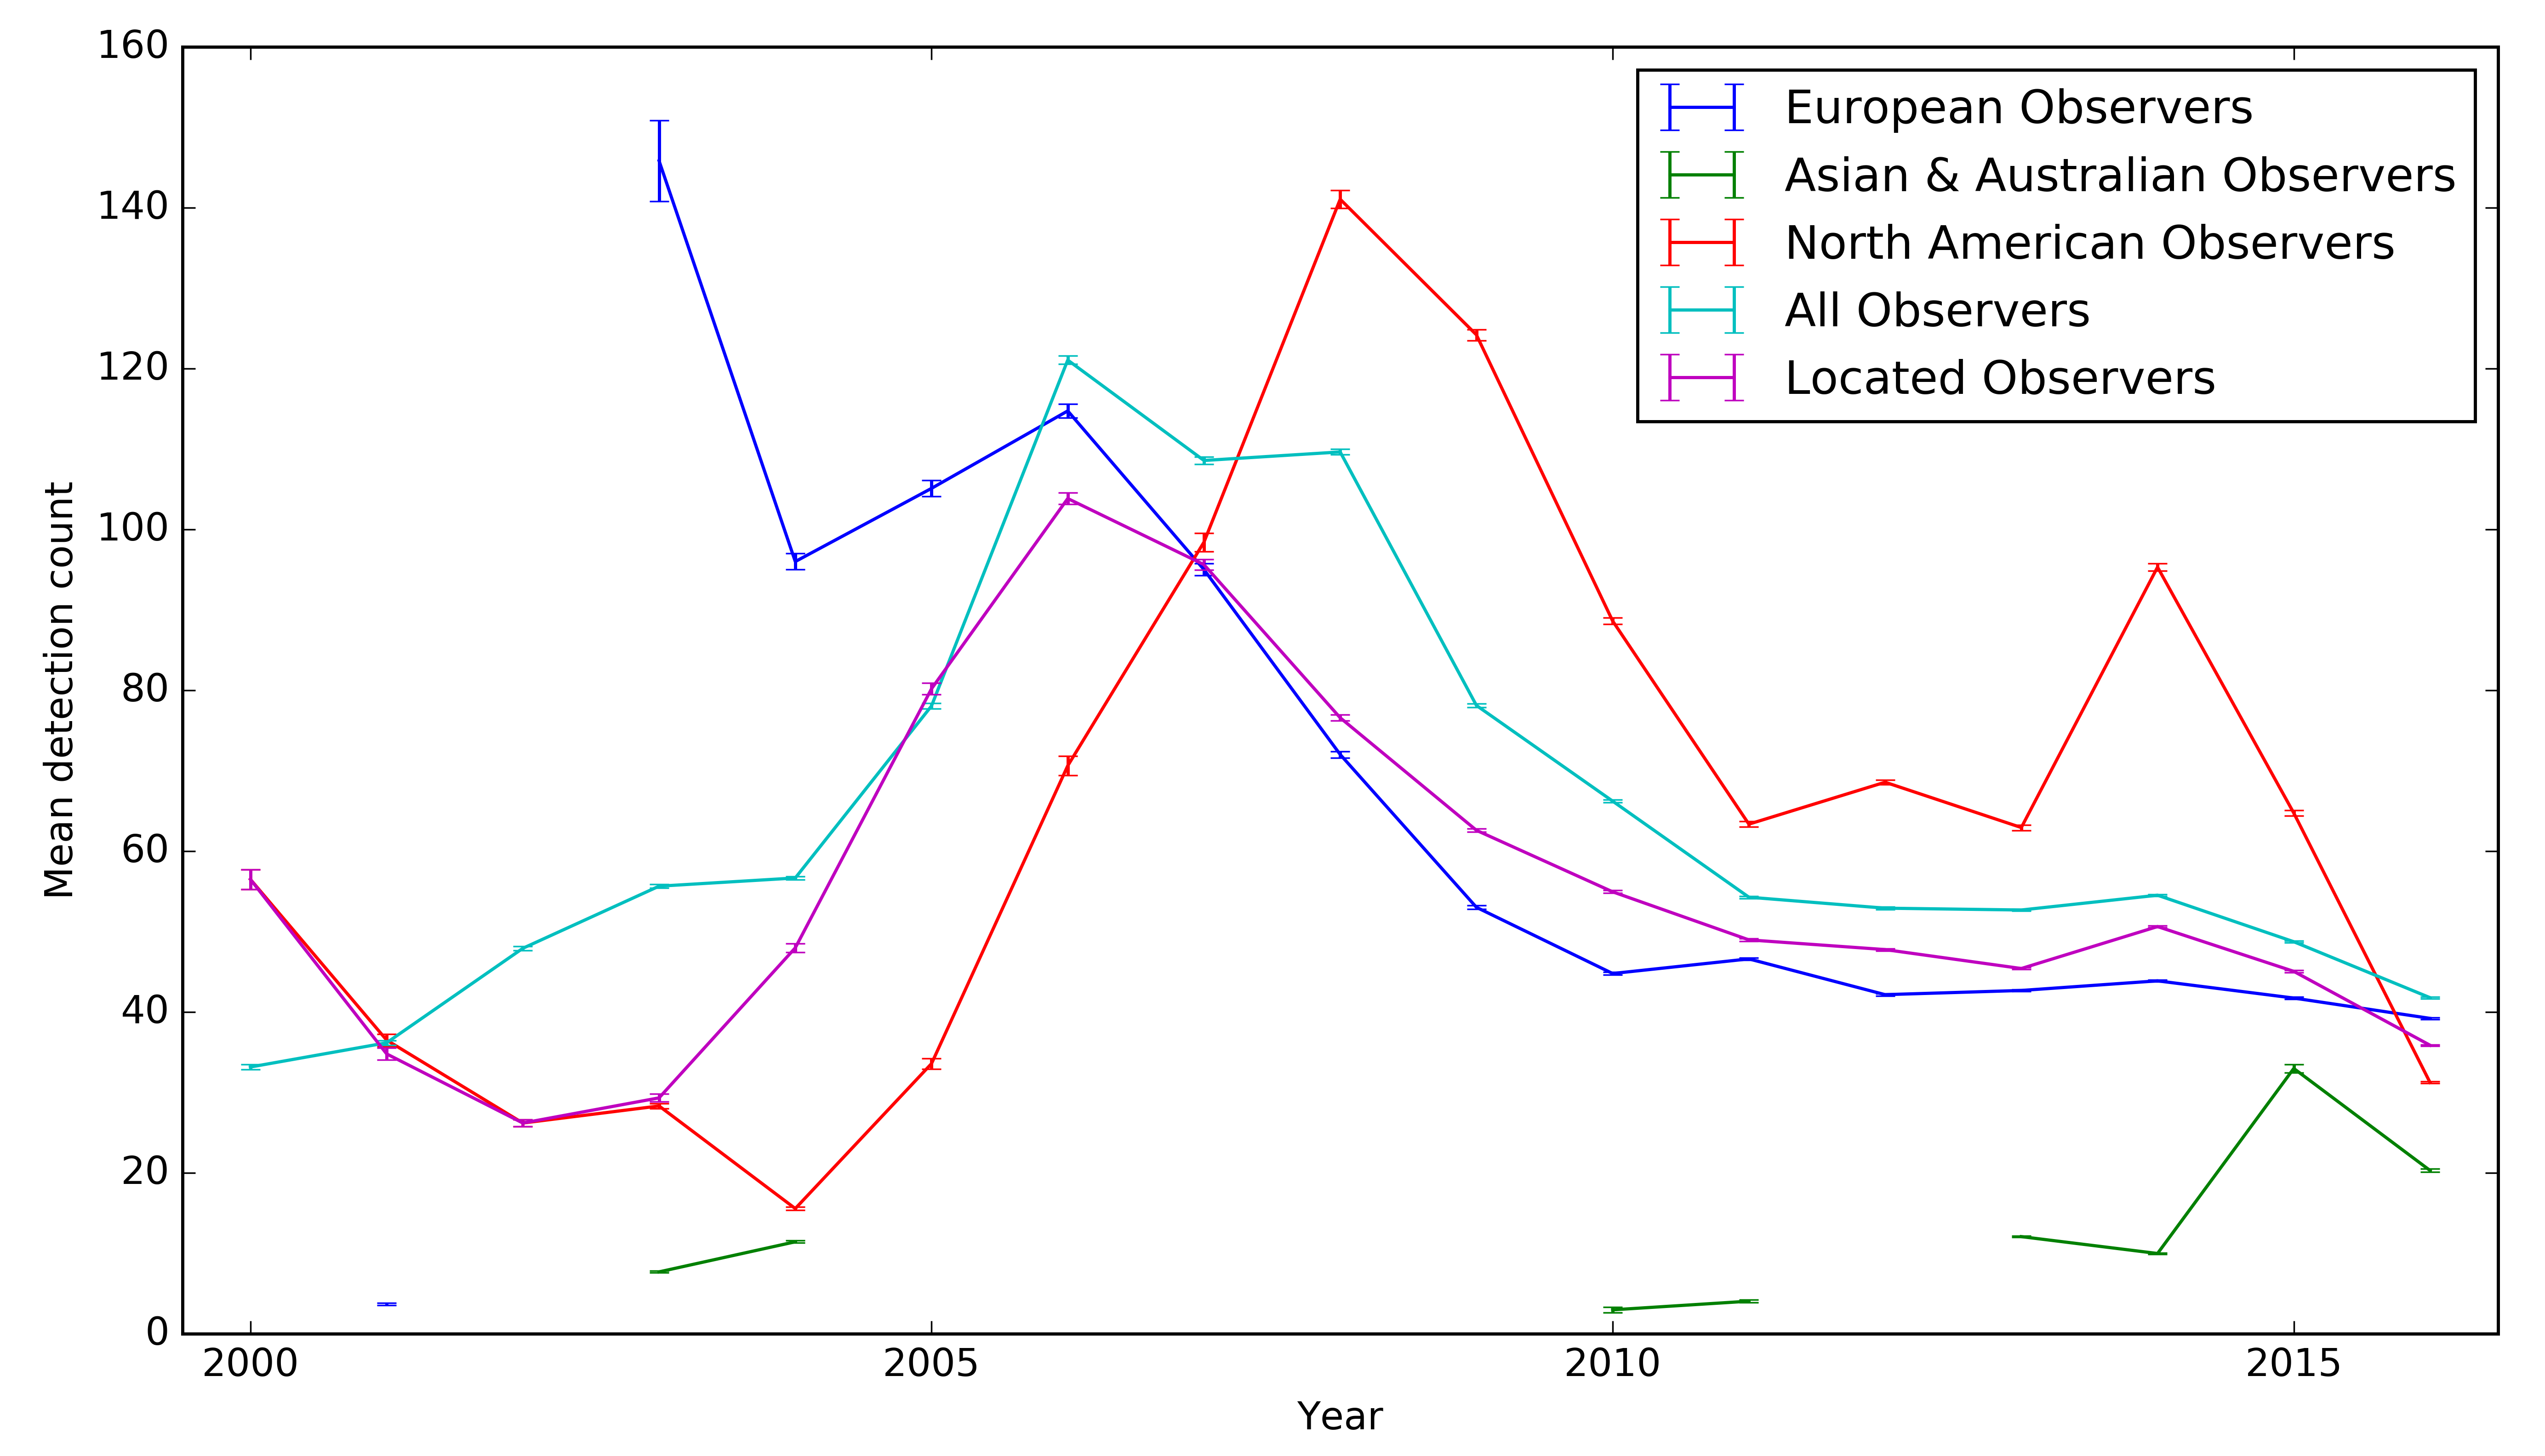
\includegraphics[width=\linewidth]{temporal/Ycombined}
	\caption{Variation in mean hourly detection count since 2000 by year
		\label{fig:temp:year}}
\end{figure}
Figure~\ref{fig:temp:yearmonth} shows the same data as figure~\ref{fig:temp:year} but on a finer resolution: for each month of each year available. The same increase is seen as before, though it is clear there there is much more variation between 2004 and 2011, as noted in section~\ref{par:err}. It is clear, from 2011 onwards, that there is a periodic variation each year, with a greater hourly detection count in the middle of the year.
\begin{figure}[h!]
	\centering
	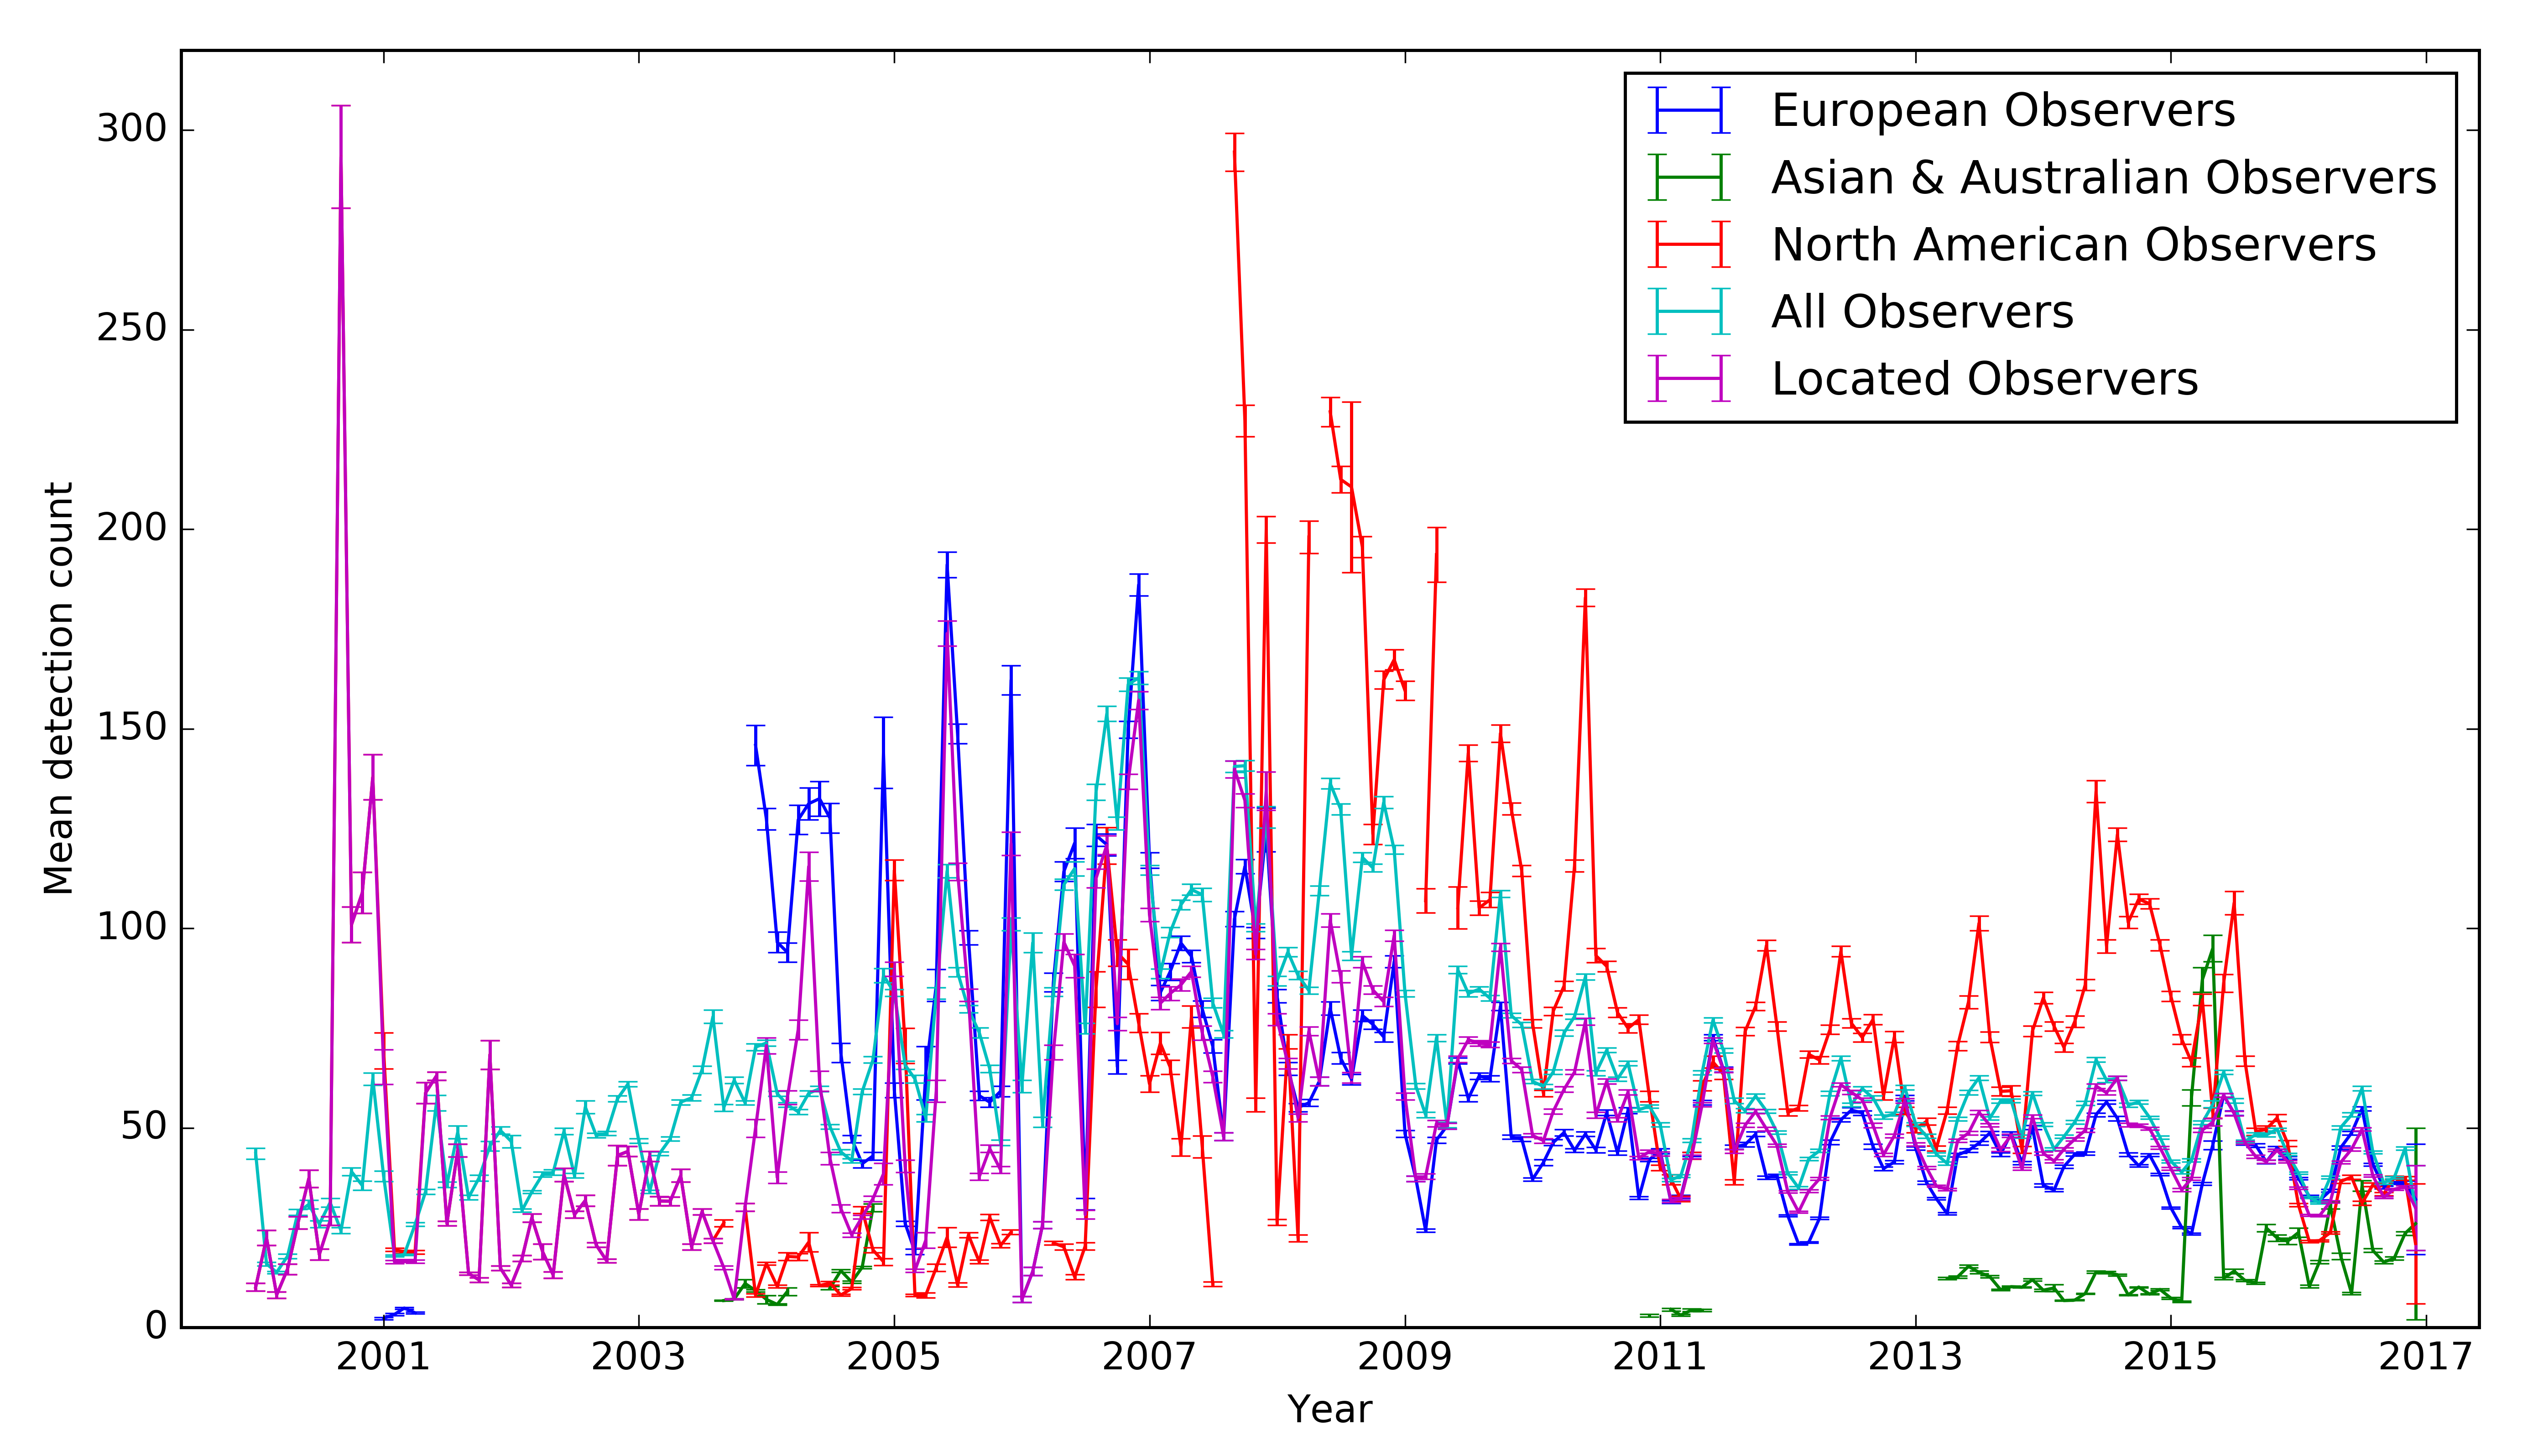
\includegraphics[width=\linewidth]{temporal/YMcombined}
	\caption{Variation in mean hourly detection count since 2000 by year and month
		\label{fig:temp:yearmonth}}
\end{figure}
\paragraph{Daytime vs. night-time rates\\}
In light of the correlation between the solar minimum and the maximum detection counts, I carried out a paired t-test to determine if there is a significant difference between the mean hourly detection counts when considering only daytime values, and night-time values. There is no significant difference between daytime and night-time (1\% significance level). 
\begin{figure*}[h!]
	\centering
	\begin{subfigure}[bh!]{0.475\textwidth}
		\centering
		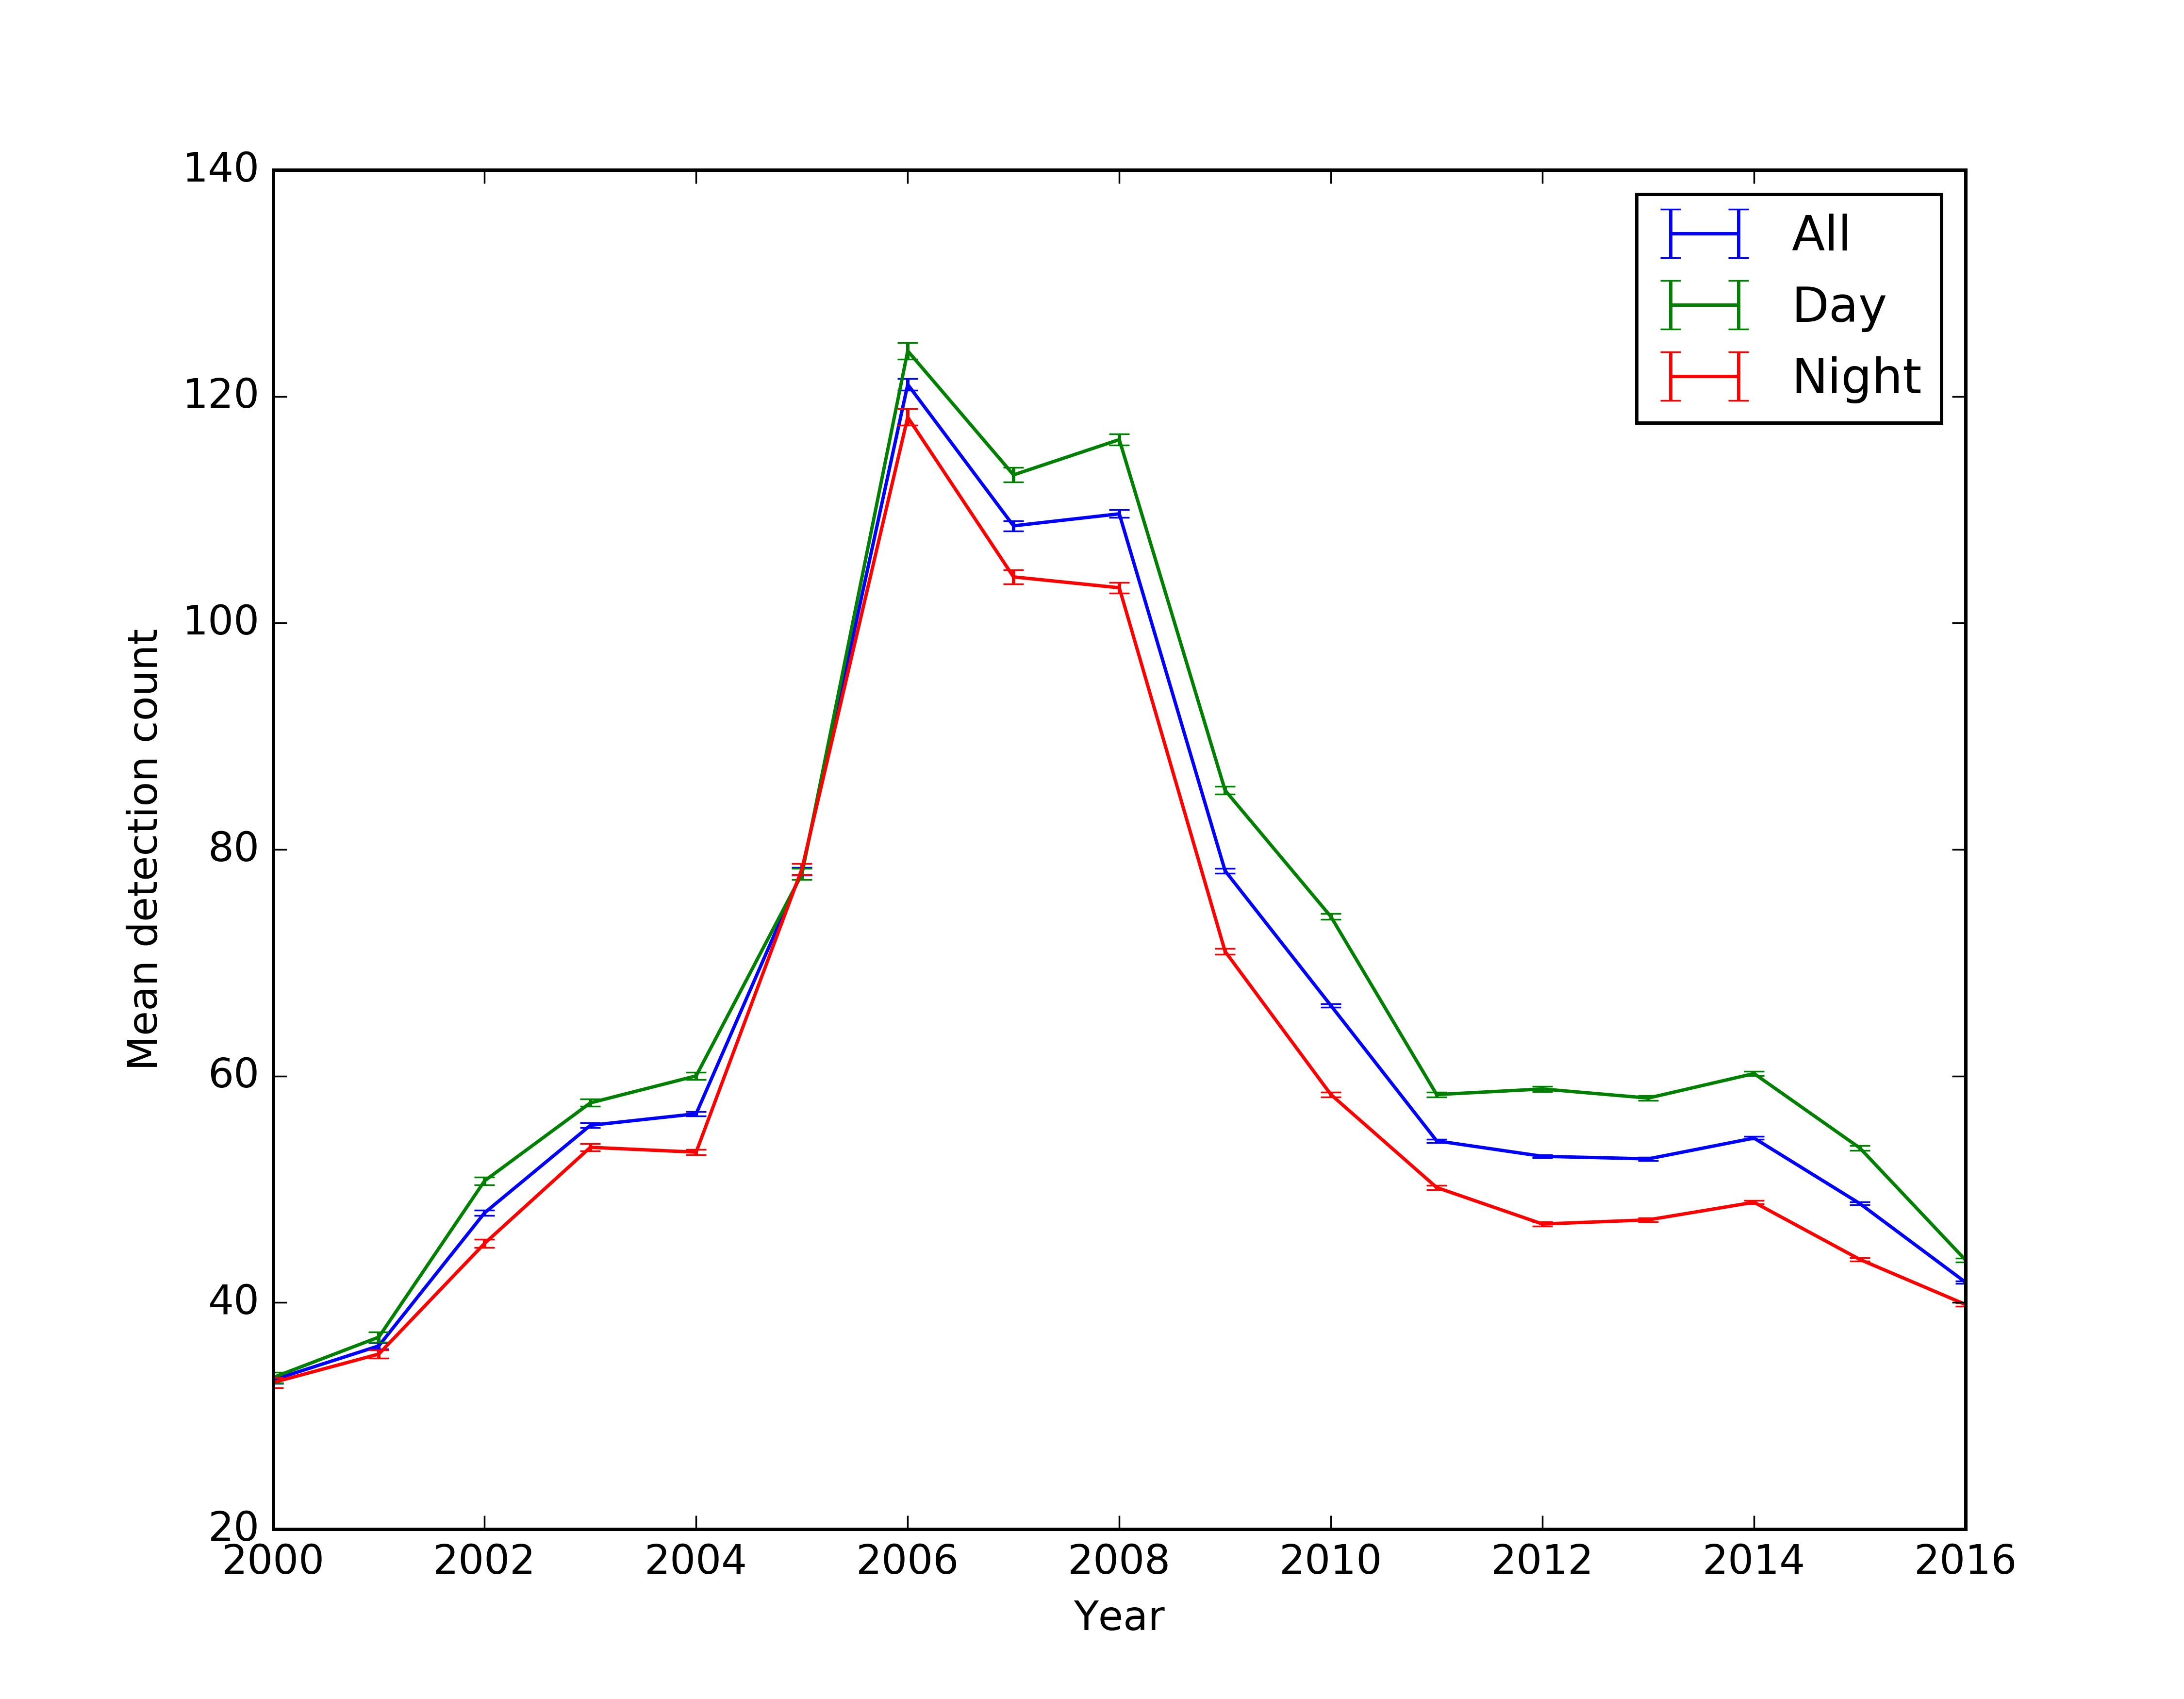
\includegraphics[width=\linewidth]{temporal/YAllcombined}
		\caption{All observers
			\label{fig:temp:daynight:a}}
	\end{subfigure}
	\hfill
	\begin{subfigure}[bh!]{0.475\textwidth}
		\centering
		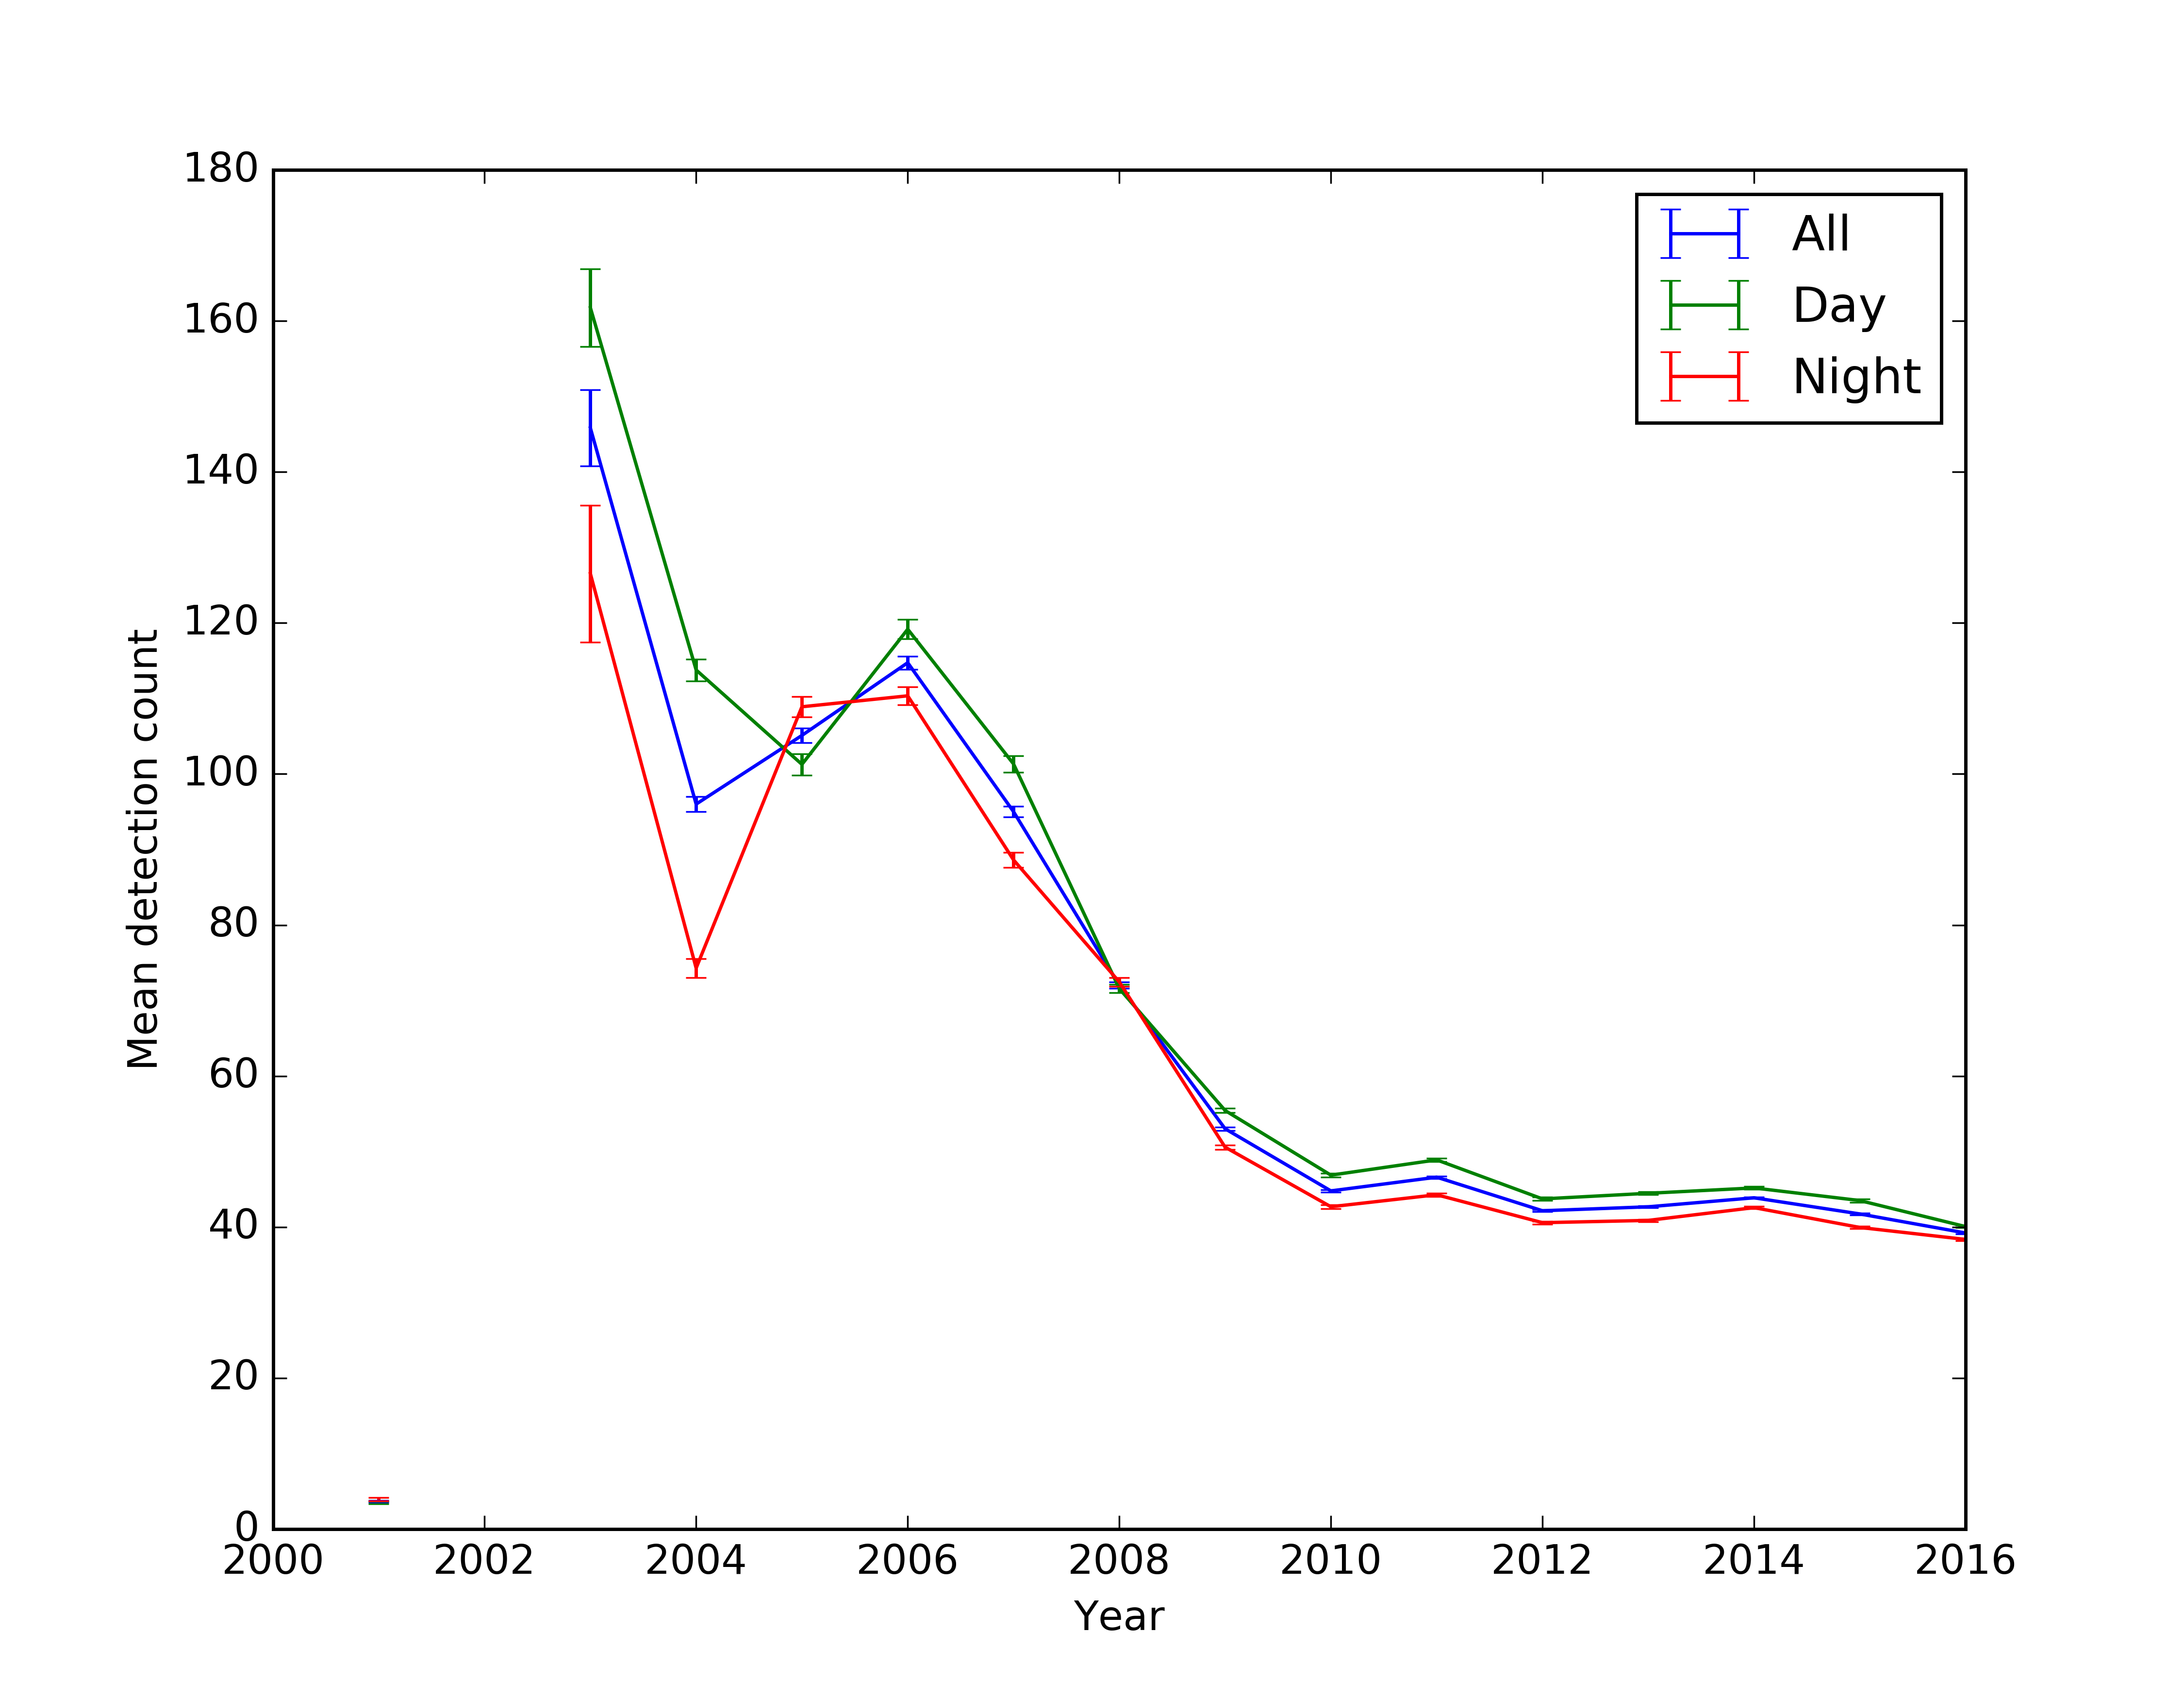
\includegraphics[width=\linewidth]{temporal/YEuropecombined}
		\caption{Observers in Europe
			\label{fig:temp:daynight:b}}
	\end{subfigure}
	\vskip\baselineskip
	\begin{subfigure}[bh!]{0.475\textwidth}
		\centering
		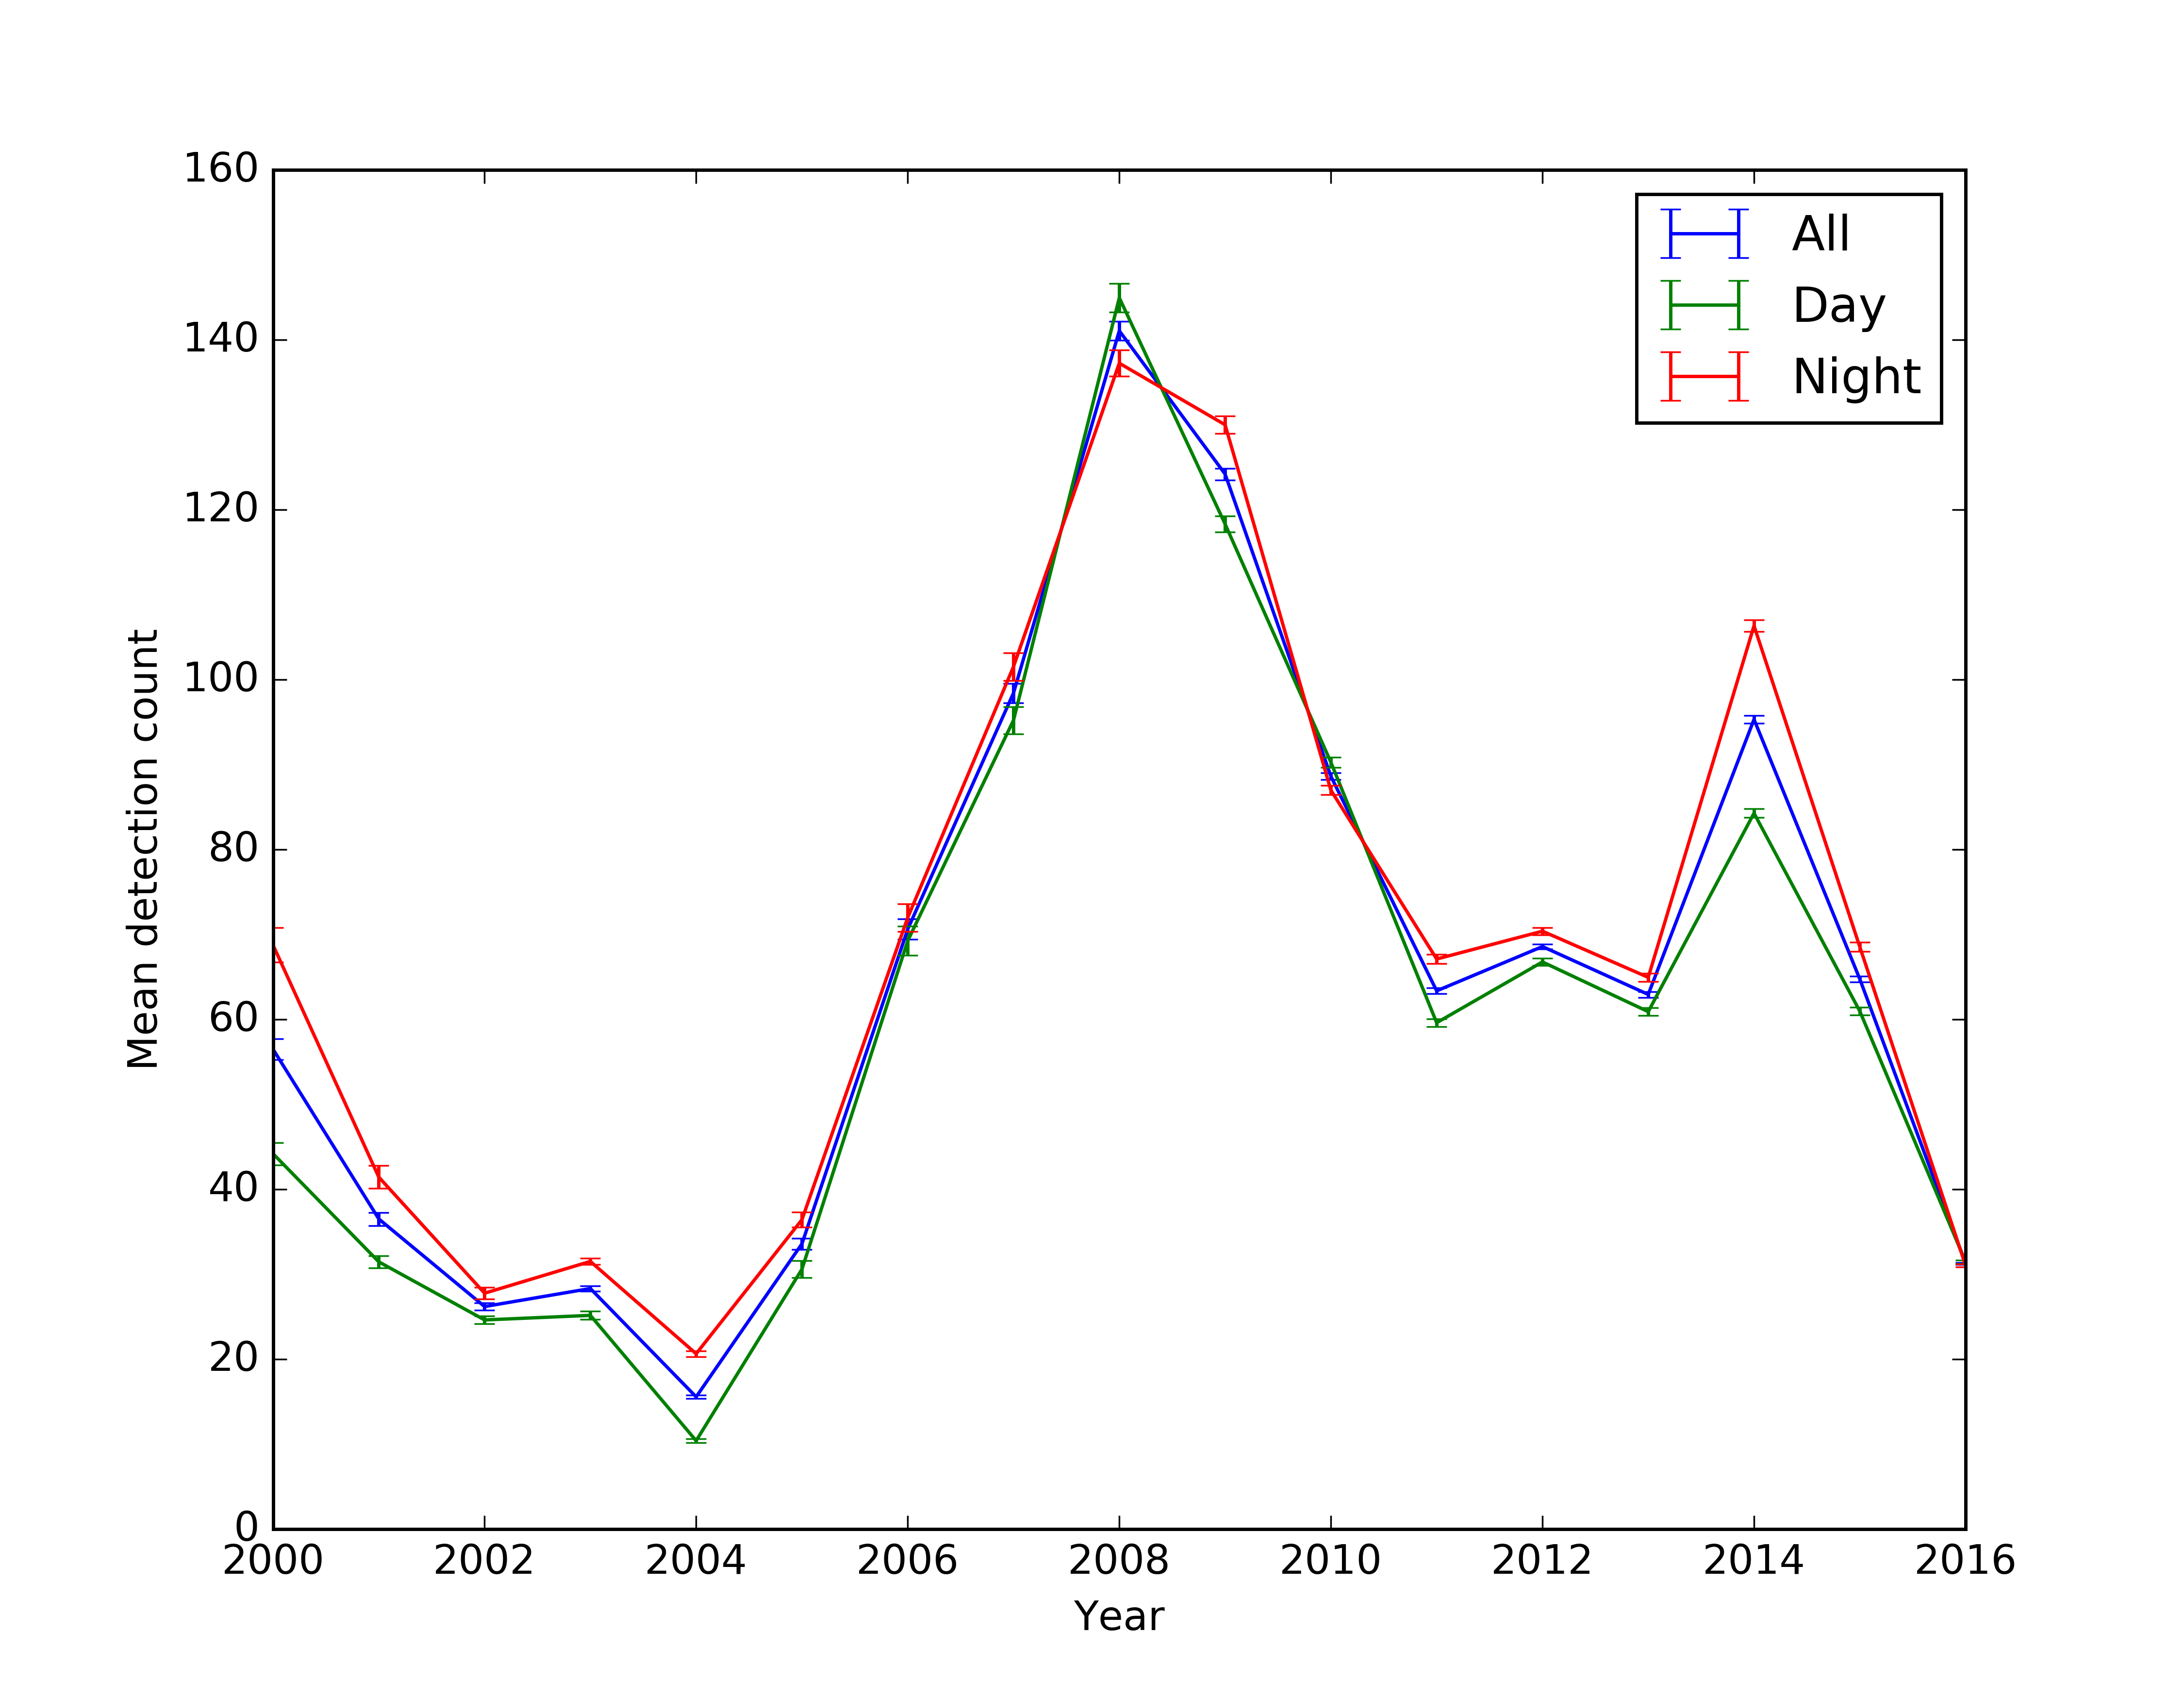
\includegraphics[width=\linewidth]{temporal/YnorthAmericaCombined}
		\caption{Observers in North America
			\label{fig:temp:daynight:c}}
	\end{subfigure}
	\quad
	\begin{subfigure}[bh!]{0.475\textwidth}
		\centering
		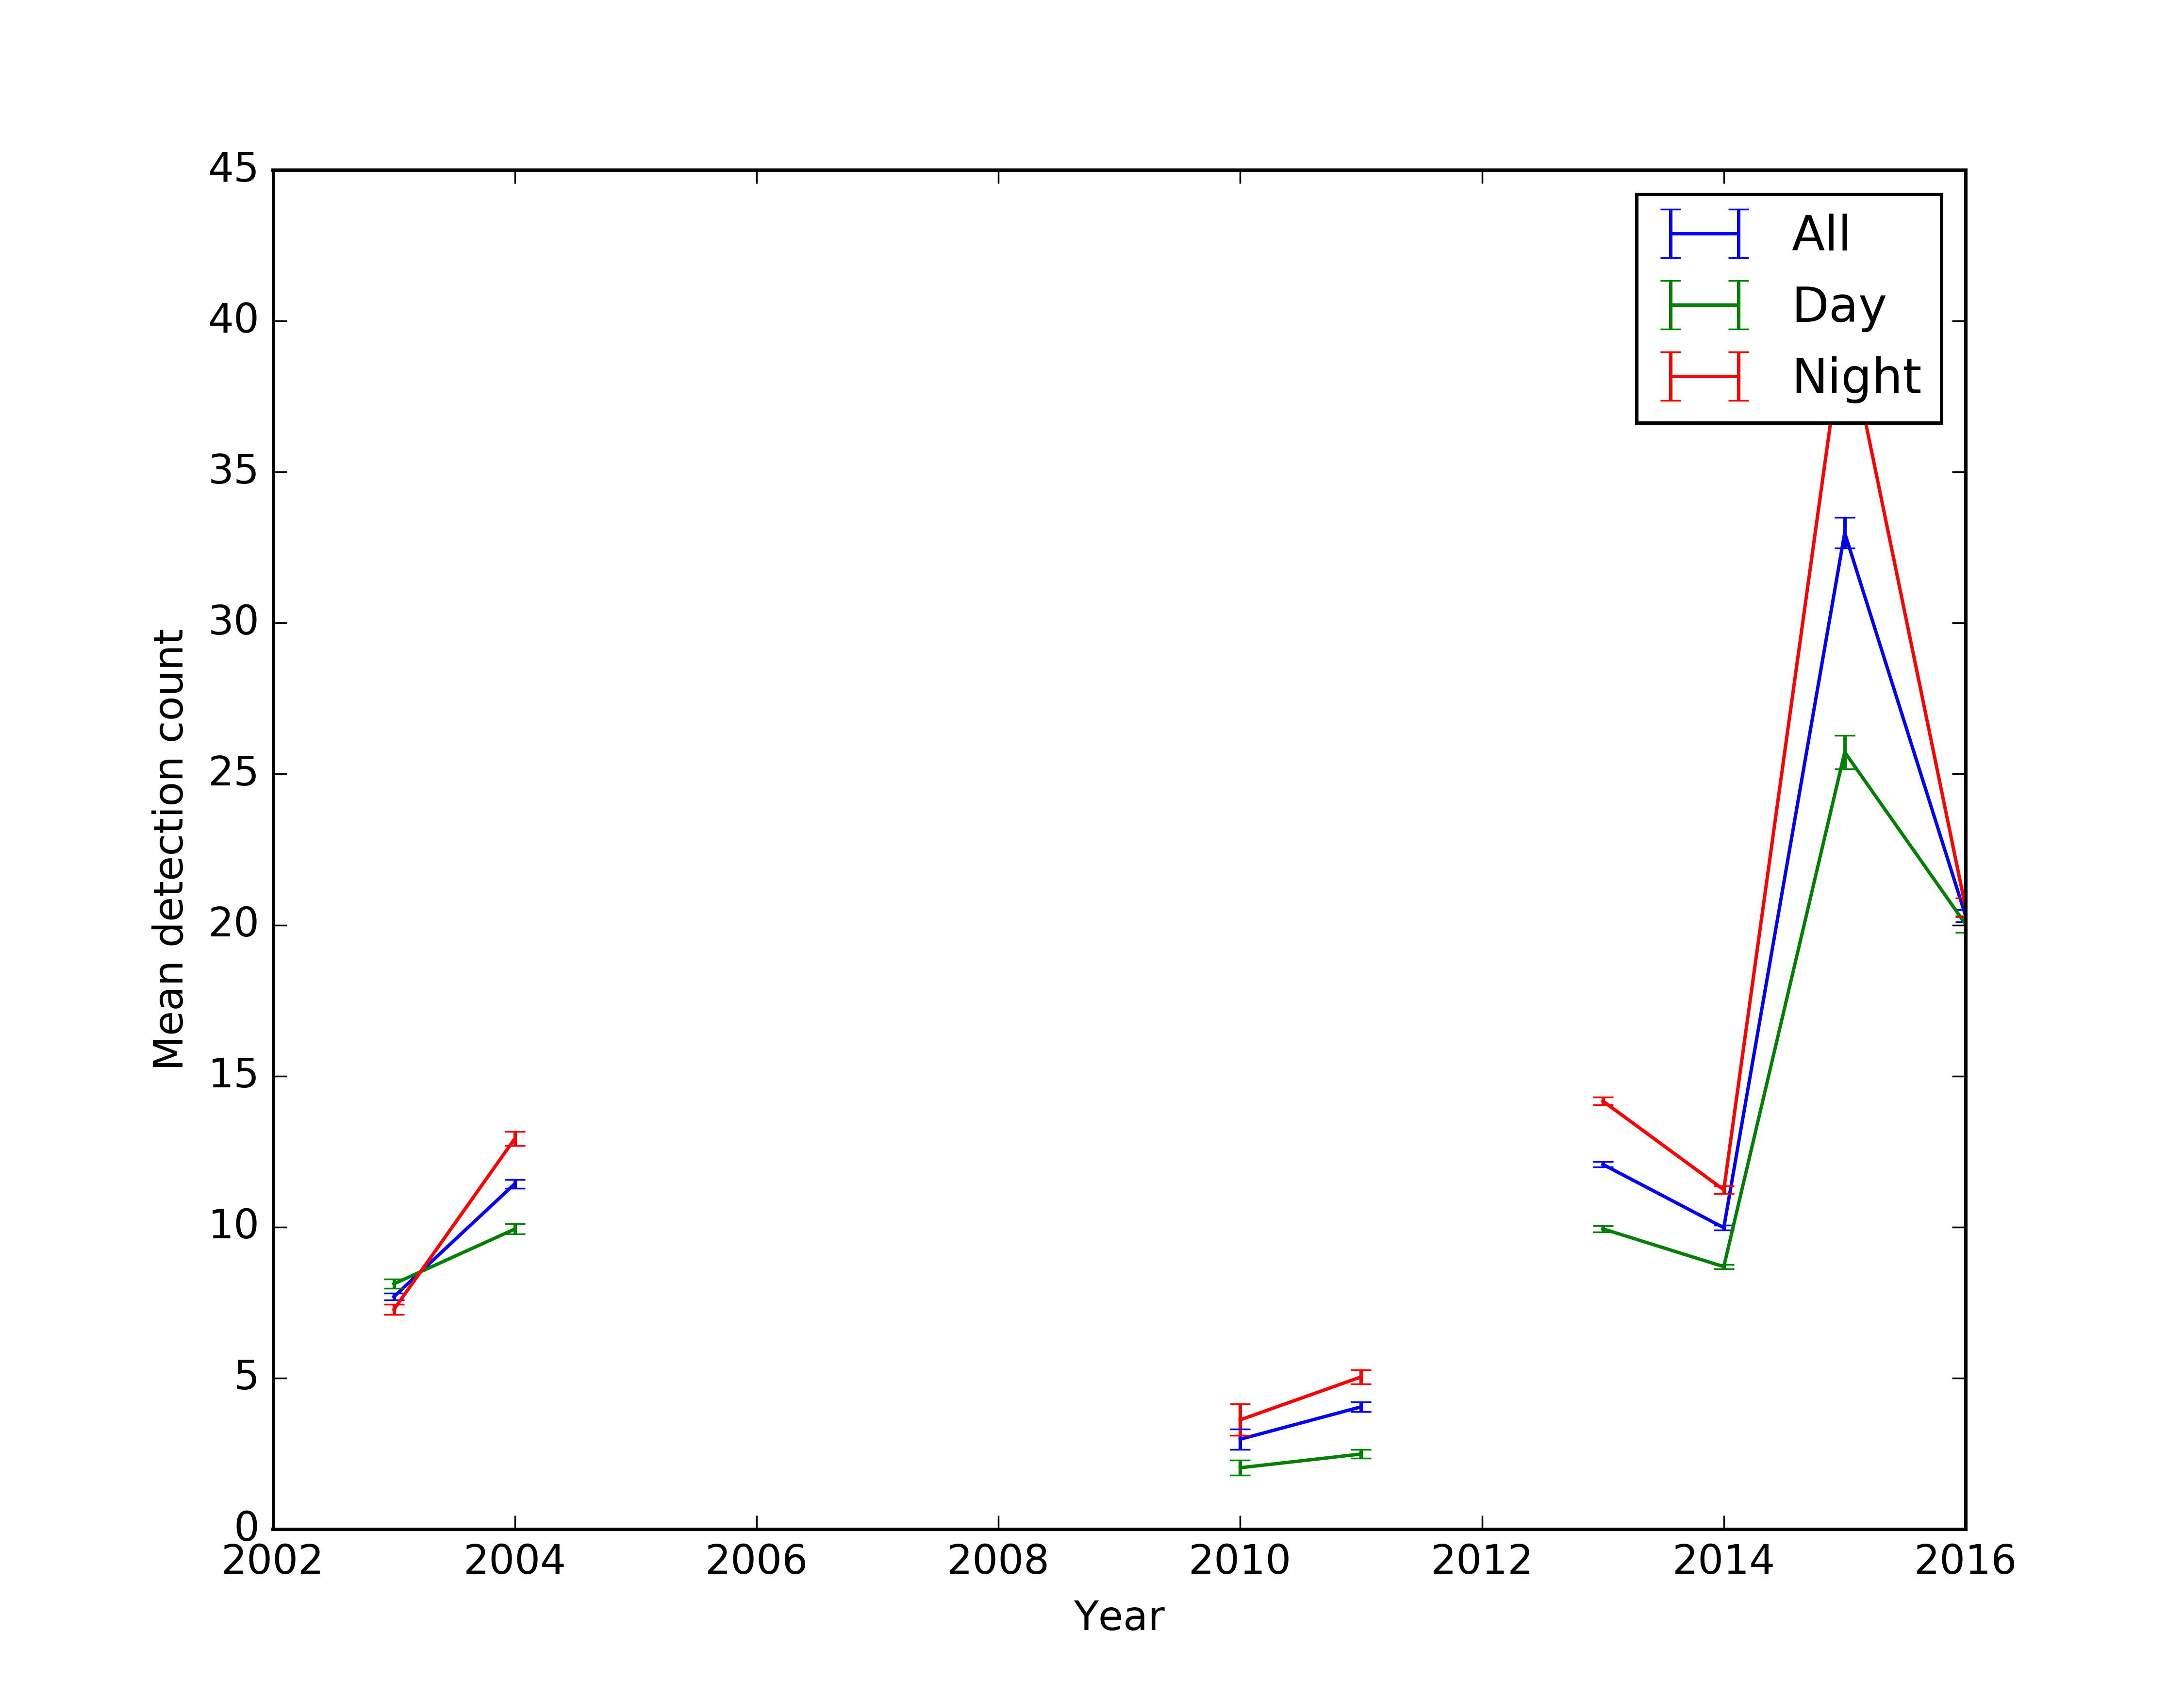
\includegraphics[width=\linewidth]{temporal/YasiaAustraliaCombined}
		\caption{Observers in Australia \& Asia
			\label{fig:temp:daynight:d}}
	\end{subfigure}
	\caption{Daytime vs. Night-time hourly detection counts}
\end{figure*}
\section{Discussion}
\subsection{Data characteristics}
\paragraph{Standard error\\}
The low variation shows that there are not large changes in hourly detection counts. This implies that influences from meteor showers do not greatly increase or decrease the detection counts, at least on a degree that would cause great variation. The increase from 2005 to 2011 agrees with figure~\ref{fig:temp:year}, where the variation greatly increases during the maximum in detection counts. The influence of a solar minimum, causing greater detection counts, supports this. With the absence of a strong solar wind, variations in the number of meteors are likely to have more effect.
\paragraph{Skewness\\}
It is expected that the skewness fluctuates around 0, primarily above 0. There will be an abrupt end in the distribution of possible detection counts since they cannot be negative, whereas there will be a tail towards large counts since there is (theoretically) no limit.
\paragraph{Diurnal shift\\}
I provide no explanation for the large amount of variation in the diurnal shift peak hour for earlier years, around 2000. In more recent years, the variation is less severe and the peak hour fluctuates around values that are expected from chapter~\ref{chap:diurnalshift}. There is a worse fit during the years where there is a maximum in detection counts, possibly because, with the greater detection counts, the diurnal shift has less influence on the total counts, meaning there is a worse fit for a sine function.
\subsection{Monthly scale variation}
It is expected that there is no overall trend over the course of a month. Any variation on this scale could potentially be caused by the moon, though it is unlikely that it would have an impact, and this is seen in the results. The small increase around the 11th-14th day of the month may be caused by a large shower, such as the Perseids, which causes such an increase in counts that it influences the mean across all months.
\subsection{Annual scale variation}
The increase in the middle of the year may be due to an increased number of meteor showers, or some other phenomenon. This increase can likely be considered part of the summer, since most observers in the sample are in the Northern Hemisphere. The low standard errors suggest that there is a clear periodic increase, and on the order of $\sim$ 20 counts an hour. The Asia \& Australia exhibits an increase, but two months earlier, and it does not persist for the rest of the year as other categories do. In chapter~\ref{chap:diurnalshift}, it appears from an analysis of fit between a sine-curve and a given observer's data that the background detection rate increases between 2005 and 2011. This result, and that presented in this chapter, appear to agree. I do not put forward any explanation for this increase; further investigation is required.
\begin{figure}[h!]
	\centering
	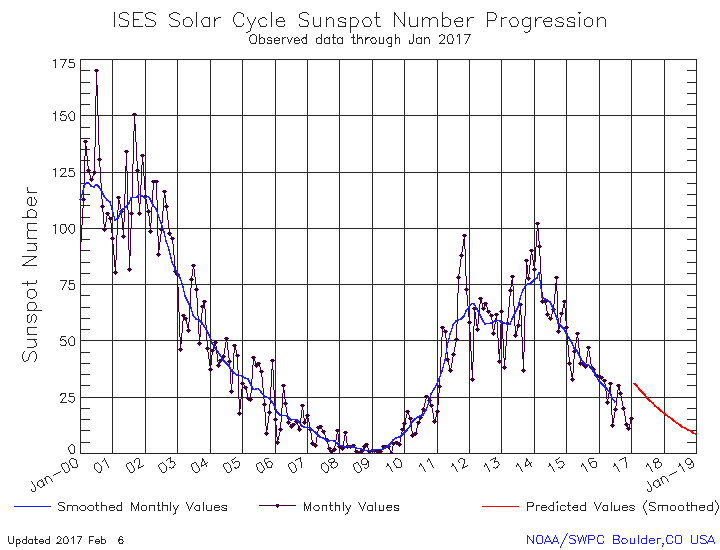
\includegraphics[width=\linewidth]{sunspots}
	\caption{Solar cycle sunspot number over time \cite{sunspot}
		\label{fig:temp:sunspot}}
\end{figure}
\subsection{Variation since 2000}
The increase centred around 2007 is significant. The maximum of the hourly detection counts occurs between 2006 and 2008, whilst the solar minimum occurs in 2009, however the sunspot number is not much larger than this from 2006, as can be seen in figure~\ref{fig:temp:sunspot}. This correlation (as well as a slight phase difference of 1 or 2 years) between solar minima and meteor maxima is noted in other articles \cite{lindblad}. That the solar cycle has an impact on meteor detection rates is not unexpected. The solar cycle influences heavily the solar wind and electron density, which will have a large influence on detection rates, especially for radio detection.
\paragraph{Daytime vs. night-time rates\\}
The fact that there is no significant difference between daytime and night-time counts seems to disagree with other studies. However, this simply rules out an influence from the Sun being above the horizon, or not. This does not discount the influence of the solar wind, since the change in electron density is not on only one side of the Earth. Thus any increase caused by the solar wind would not cause a significance difference between daytime and night-time counts. Theoretically, the peak hour of diurnal shift occurs at Sunset, so any influence will be uniform between day and night, so this can be disregarded.
\section{Conclusion}
I have found a significant increase in hourly detection counts between 2005 and 2011. The increase correlates well with solar activity, which supports hypothesis from Lindblad and Bumbda, as cited in section~\ref{sec:temp:litrev}. There is no basis to reject the hypothesis that the daytime and night-time hourly detection counts are different (1\% significance level), indicating that there is no influence on detection counts that varies over a single day's time frame. The results also show an increase in the middle of the year, which I provide no full explanation for. Further work on a hemispherical analysis may provide more information on this. A combination of a temporal and spacial analysis may also provide more information, since the two `dimensions' of variation often work in conjunction with one another.